% !TeX encoding = UTF-8
% !TeX root = V30_Nonlinear.tex
% !TeX spellcheck = en_US

\section{Execution}
\subsection{Measurements of the diode laser}
\subsubsection{Diode laser: Detected power $P(I,T)$}
In order to determine the power output of a diode laser, we measure the power of the emitted beam with a photo detector. The experimental setup is depicted in figure \ref{fig:setup_P}. It is set to detect a particular wavelength $\lambda$, since the diode laser emits a beam with a continuous spectrum and only a certain wavelength (see theory) is used to pump the active medium (Nd:YAG) later on. The power output mostly depends on the injection current $I$ and the temperature $T$ within the laser diode.

\begin{figure}[h]
	\centering
	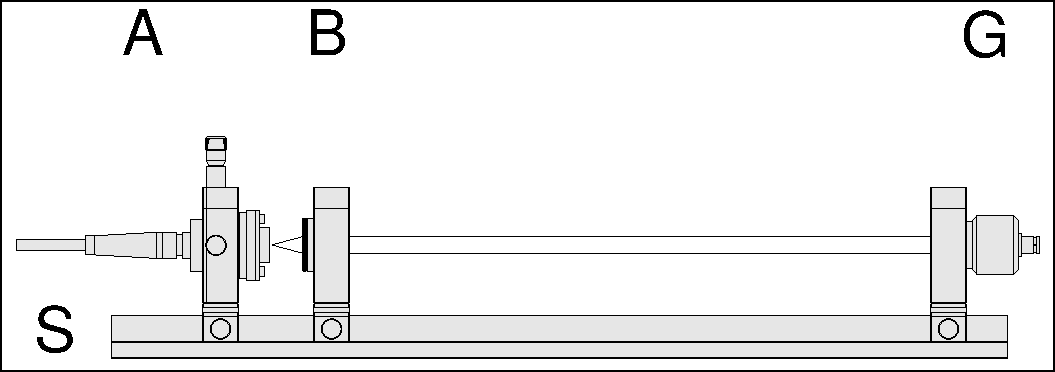
\includegraphics[width=0.9\textwidth]{setup_P.pdf}
	\caption[Measurement of the diode laser power]{Experimental setup for measuring the output power of the diode laser. The diode laser acts as a point source of light (A). The initially strongly divergent beam passes through a collimator (B) and then hits a photo detector (G) with a connected device, which shows us the detected power $P$ at a certain wavelength $\lambda$. All optical devices are set upon a optical bank (S) in all subsequent experimental setups. \cite{lit:manual}}
	\label{fig:setup_P}
\end{figure}

The injection currents $I$ and the temperatures $T$ are chosen such that
\begin{align*}
I=&0,40,80,\dots,200\milli\ampere\\
I=&200,220,240,\dots,500\milli\ampere\\
T=&15,17,19,\dots,35\celsius.
\end{align*}
The measured powers are plotted against $I$ for various $T$ in figure \ref{fig:measurement_P}.

\begin{figure}[h]
	\centering
	% This file was created by matlab2tikz.
% Minimal pgfplots version: 1.3
%
\definecolor{mycolor1}{rgb}{0.00000,0.75000,0.75000}%
\definecolor{mycolor2}{rgb}{0.75000,0.00000,0.75000}%
\definecolor{mycolor3}{rgb}{0.75000,0.75000,0.00000}%
%
\begin{tikzpicture}

\begin{axis}[%
width=0.855828\textwidth,
height=0.675\textwidth,
at={(0\textwidth,0\textwidth)},
scale only axis,
separate axis lines,
every outer x axis line/.append style={black},
every x tick label/.append style={font=\color{black}},
xmin=0,
xmax=500,
xlabel={Injection current $I(\milli\ampere)$},
every outer y axis line/.append style={black},
every y tick label/.append style={font=\color{black}},
ymin=0,
ymax=180,
ylabel={Detected photo detector power $P(\milli\watt)$},
legend style={at={(0.03,0.97)},anchor=north west,legend cell align=left,align=left,draw=black}
]
\addplot [color=blue,solid]
  table[row sep=crcr]{%
0	5e-05\\
40	0.0052\\
80	0.0223\\
120	0.058\\
160	0.178\\
200	2.2\\
220	11.5\\
240	21\\
260	32.7\\
280	43\\
300	54.5\\
320	65.3\\
340	74.6\\
360	85.3\\
380	96.5\\
400	108\\
420	118.1\\
440	129.6\\
460	141.2\\
480	151.8\\
500	162.6\\
};
\addlegendentry{$15\celsius$};

\addplot [color=black!50!green,solid]
  table[row sep=crcr]{%
0	5e-05\\
40	0.0055\\
80	0.0226\\
120	0.0596\\
160	0.181\\
200	1.45\\
220	10.9\\
240	22.5\\
260	32.2\\
280	42.9\\
300	55.1\\
320	64.3\\
340	75.7\\
360	85\\
380	95.5\\
400	106.8\\
420	118.1\\
440	129\\
460	140.9\\
480	152\\
500	162.8\\
};
\addlegendentry{$17\celsius$};

\addplot [color=red,solid]
  table[row sep=crcr]{%
0	5e-05\\
40	0.0057\\
80	0.023\\
120	0.061\\
160	0.181\\
200	1.3\\
220	10.45\\
240	22\\
260	32.3\\
280	42.8\\
300	53.9\\
320	64.6\\
340	74.4\\
360	85.2\\
380	96.1\\
400	106.6\\
420	117.5\\
440	128\\
460	139\\
480	150.6\\
500	162\\
};
\addlegendentry{$19\celsius$};

\addplot [color=mycolor1,solid]
  table[row sep=crcr]{%
0	5e-05\\
40	0.006\\
80	0.0234\\
120	0.0589\\
160	0.172\\
200	0.81\\
220	9\\
240	19.6\\
260	30.5\\
280	40.5\\
300	51.6\\
320	61.9\\
340	73.2\\
360	83.3\\
380	93.3\\
400	104.6\\
420	115.5\\
440	126.1\\
460	137.6\\
480	148.9\\
500	160.4\\
};
\addlegendentry{$21\celsius$};

\addplot [color=mycolor2,solid]
  table[row sep=crcr]{%
0	5e-05\\
40	0.0057\\
80	0.0231\\
120	0.059\\
160	0.165\\
200	0.712\\
220	8.3\\
240	18.9\\
260	29.7\\
280	39.6\\
300	50.7\\
320	61.6\\
340	71.9\\
360	82.8\\
380	93\\
400	103.3\\
420	114.2\\
440	125.2\\
460	136.4\\
480	147.5\\
500	158.7\\
};
\addlegendentry{$23\celsius$};

\addplot [color=mycolor3,solid]
  table[row sep=crcr]{%
0	5e-05\\
40	0.0055\\
80	0.0233\\
120	0.0751\\
160	0.16\\
200	0.675\\
220	7.3\\
240	17.6\\
260	28.7\\
280	38.4\\
300	49.6\\
320	60.1\\
340	70.4\\
360	81.5\\
380	91.1\\
400	102.1\\
420	112.2\\
440	124.2\\
460	135.1\\
480	145.9\\
500	157.7\\
};
\addlegendentry{$25\celsius$};

\addplot [color=darkgray,solid]
  table[row sep=crcr]{%
0	5e-05\\
40	0.00594\\
80	0.0229\\
120	0.0569\\
160	0.158\\
200	0.603\\
220	6.4\\
240	16.6\\
260	27.2\\
280	37.8\\
300	48.1\\
320	59.2\\
340	70.3\\
360	80.5\\
380	90.6\\
400	101.5\\
420	112\\
440	122.7\\
460	133.8\\
480	144.8\\
500	156\\
};
\addlegendentry{$27\celsius$};

\addplot [color=blue,solid]
  table[row sep=crcr]{%
0	5e-05\\
40	0.0061\\
80	0.0236\\
120	0.0578\\
160	0.155\\
200	0.55\\
220	5.1\\
240	15.2\\
260	26.3\\
280	36.8\\
300	47\\
320	57.8\\
340	68.9\\
360	80\\
380	90.2\\
400	100.2\\
420	110.9\\
440	121.4\\
460	133\\
480	144.1\\
500	155.1\\
};
\addlegendentry{$29\celsius$};

\addplot [color=black!50!green,solid]
  table[row sep=crcr]{%
0	5e-05\\
40	0.0065\\
80	0.0244\\
120	0.0588\\
160	0.157\\
200	0.55\\
220	5.4\\
240	14.5\\
260	25.8\\
280	36.3\\
300	47\\
320	57.9\\
340	68.9\\
360	79.7\\
380	90.1\\
400	100.6\\
420	110.7\\
440	122\\
460	133.1\\
480	143.5\\
500	155.2\\
};
\addlegendentry{$31\celsius$};

\addplot [color=red,solid]
  table[row sep=crcr]{%
0	5e-05\\
40	0.0061\\
80	0.0232\\
120	0.055\\
160	0.145\\
200	0.478\\
220	2.9\\
240	12.4\\
260	23.4\\
280	34.3\\
300	44\\
320	55.1\\
340	66.1\\
360	77.1\\
380	87.7\\
400	98.1\\
420	107.9\\
440	118.7\\
460	130.1\\
480	140.7\\
500	151.8\\
};
\addlegendentry{$33\celsius$};

\addplot [color=mycolor1,solid]
  table[row sep=crcr]{%
0	5e-05\\
40	0.0061\\
80	0.0226\\
120	0.0537\\
160	0.141\\
200	0.445\\
220	1.5\\
240	10.8\\
260	22.3\\
280	32.6\\
300	42.5\\
320	53\\
340	64.6\\
360	76.5\\
380	85.7\\
400	96.2\\
420	106.5\\
440	117.7\\
460	128.6\\
480	138.8\\
500	150.1\\
};
\addlegendentry{$35\celsius$};

\end{axis}
\end{tikzpicture}%
	\caption{Detected laser diode power $P(I,T)$.}
	\label{fig:measurement_P}
\end{figure}

We can assume the increase of power $P(I,T)$ is linear to $I$, above a particular \emph{threshold} current, which is approx. $I_\text{min}=200\milli\ampere$, depending on the temperature $T$ as well. The average slope $m_1$ , computed from linear regression of all the plots, is
\begin{align}
m_1=(0,5356\pm 0,0030)\tfrac{\milli\watt}{\milli\ampere}.
\label{eq:avg_slope1}
\end{align}
This can be used for further measurements and calculations.
We can also see the power $P$ is decreasing with rising temperature $T$, also shifting the threshold current $I_\text{min}$ to slightly higher values. This could be further evaluated with more data points in the relevant current range.
A possible reason for this power decrease is the broadening of the stimulated emission energy distribution. Since we only measure the mean of this distribution, and the total energy stays the same, the peak power is lower.
\subsubsection{Diode laser: Emitted wavelength $\lambda(I,T)$}
\label{sec:diode_laser_lambda}
The next step is to determine the emitted wavelength $\lambda(I,T)$ of the diode laser, which is also dependent on the injection current $I$ and the temperature $T$. This is mostly due to the change of the refractive index in the active medium with a higher charge carrier density, and semi-conductors are very temperature-dependent in general.
The setup for this measurement is the same as shown in figure \ref{fig:setup_P}. The photo detector is swapped for a different one with a adjustable semi-transparent bar to reduce the radiation power onto the detector. It is connected to a wavemeter, which gives us a wavelength $\lambda$.
Measurements for currents $I=200,220,\dots,500\milli\ampere$ and temperatures $T=15,17,\dots,35\celsius$ are plotted in figure \ref{fig:lambda1}.

\begin{figure}[h]
	\centering
	% This file was created by matlab2tikz.
% Minimal pgfplots version: 1.3
%
\definecolor{mycolor1}{rgb}{0.00000,0.75000,0.75000}%
\definecolor{mycolor2}{rgb}{0.75000,0.00000,0.75000}%
\definecolor{mycolor3}{rgb}{0.75000,0.75000,0.00000}%
%
\begin{tikzpicture}

\begin{axis}[%
width=0.565951\textwidth,
height=0.675\textwidth,
at={(0\textwidth,0\textwidth)},
scale only axis,
unbounded coords=jump,
separate axis lines,
every outer x axis line/.append style={black},
every x tick label/.append style={font=\color{black}},
xmin=200,
xmax=500,
xlabel={Injection current $I(\milli\ampere)$},
every outer y axis line/.append style={black},
every y tick label/.append style={font=\color{black}},
ymin=803,
ymax=810,
ylabel={Wavelength $\lambda(\nano\metre)$},
legend style={at={(1.03,1)},anchor=north west,legend cell align=left,align=left,draw=black}
]
\addplot [color=blue,mark size=4.0pt,only marks,mark=x,mark options={solid}]
  table[row sep=crcr]{%
200	803.05\\
220	803.15\\
240	803.75\\
260	803.3\\
280	803.4\\
300	803.95\\
320	803.55\\
340	803.75\\
360	803.85\\
380	804.15\\
400	804.15\\
420	803.85\\
440	804.1\\
460	803.75\\
480	803.95\\
500	804.05\\
};
\addlegendentry{$15\celsius$};

\addplot [color=black!50!green,mark size=4.0pt,only marks,mark=x,mark options={solid}]
  table[row sep=crcr]{%
200	803.75\\
220	804.05\\
240	804.25\\
260	804.25\\
280	804.25\\
300	804.25\\
320	804.25\\
340	804.4\\
360	804.25\\
380	804.4\\
400	804.4\\
420	804.65\\
440	804.45\\
460	804.85\\
480	804.6\\
500	804.6\\
};
\addlegendentry{$17\celsius$};

\addplot [color=red,mark size=4.0pt,only marks,mark=x,mark options={solid}]
  table[row sep=crcr]{%
200	804.1\\
220	804.35\\
240	805.1\\
260	804.5\\
280	805\\
300	805.1\\
320	804.65\\
340	805.1\\
360	805\\
380	805.2\\
400	805.4\\
420	805.1\\
440	805.3\\
460	805.25\\
480	805.05\\
500	805.35\\
};
\addlegendentry{$19\celsius$};

\addplot [color=mycolor1,mark size=4.0pt,only marks,mark=x,mark options={solid}]
  table[row sep=crcr]{%
200	804.8\\
220	805\\
240	805.15\\
260	805.2\\
280	805.35\\
300	805.3\\
320	805.2\\
340	805.15\\
360	805.3\\
380	805.15\\
400	805.75\\
420	805.55\\
440	805.65\\
460	805.7\\
480	805.9\\
500	805.75\\
};
\addlegendentry{$21\celsius$};

\addplot [color=mycolor2,mark size=4.0pt,only marks,mark=x,mark options={solid}]
  table[row sep=crcr]{%
200	nan\\
220	805.95\\
240	805.95\\
260	805.8\\
280	806.1\\
300	805.95\\
320	805.9\\
340	806.35\\
360	805.65\\
380	806.3\\
400	805.65\\
420	806.45\\
440	806.25\\
460	806\\
480	806.25\\
500	806.25\\
};
\addlegendentry{$23\celsius$};

\addplot [color=mycolor3,mark size=4.0pt,only marks,mark=x,mark options={solid}]
  table[row sep=crcr]{%
200	nan\\
220	806.15\\
240	806.15\\
260	806.25\\
280	806.25\\
300	806.15\\
320	806.25\\
340	806.4\\
360	806.3\\
380	806.7\\
400	806.7\\
420	806.65\\
440	806.65\\
460	807.05\\
480	806.8\\
500	806.8\\
};
\addlegendentry{$25\celsius$};

\addplot [color=darkgray,mark size=4.0pt,only marks,mark=x,mark options={solid}]
  table[row sep=crcr]{%
200	nan\\
220	806.4\\
240	806.65\\
260	807.3\\
280	807\\
300	806.8\\
320	807.25\\
340	806.65\\
360	807.25\\
380	807.35\\
400	807.3\\
420	807.25\\
440	807.25\\
460	807.25\\
480	807.4\\
500	807.2\\
};
\addlegendentry{$27\celsius$};

\addplot [color=blue,mark size=4.0pt,only marks,mark=x,mark options={solid}]
  table[row sep=crcr]{%
200	nan\\
220	807.1\\
240	807.2\\
260	807.4\\
280	807.3\\
300	807.5\\
320	807.7\\
340	807.25\\
360	807.6\\
380	807.6\\
400	808.1\\
420	807.95\\
440	807.65\\
460	808\\
480	807.85\\
500	808.1\\
};
\addlegendentry{$29\celsius$};

\addplot [color=black!50!green,mark size=4.0pt,only marks,mark=x,mark options={solid}]
  table[row sep=crcr]{%
200	nan\\
220	807.75\\
240	807.65\\
260	808.2\\
280	808\\
300	808.25\\
320	808.3\\
340	807.7\\
360	808.2\\
380	808.35\\
400	808.45\\
420	808.25\\
440	808.25\\
460	808.2\\
480	808.45\\
500	808.65\\
};
\addlegendentry{$31\celsius$};

\addplot [color=red,mark size=4.0pt,only marks,mark=x,mark options={solid}]
  table[row sep=crcr]{%
200	nan\\
220	808.05\\
240	808.15\\
260	809.25\\
280	808.5\\
300	808.3\\
320	808.65\\
340	808.6\\
360	808.35\\
380	808.9\\
400	809\\
420	809\\
440	808.9\\
460	808.6\\
480	808.7\\
500	809.3\\
};
\addlegendentry{$33\celsius$};

\addplot [color=mycolor1,mark size=4.0pt,only marks,mark=x,mark options={solid}]
  table[row sep=crcr]{%
200	nan\\
220	808.75\\
240	809\\
260	809.1\\
280	808.5\\
300	809.45\\
320	809.15\\
340	809.35\\
360	809.2\\
380	809.35\\
400	809.45\\
420	809.55\\
440	809.5\\
460	809.45\\
480	809.55\\
500	809.4\\
};
\addlegendentry{$35\celsius$};

\addplot [color=blue,solid,forget plot]
  table[row sep=crcr]{%
200	803.308088235294\\
220	803.364926470588\\
240	803.421764705882\\
260	803.478602941177\\
280	803.535441176471\\
300	803.592279411765\\
320	803.649117647059\\
340	803.705955882353\\
360	803.762794117647\\
380	803.819632352941\\
400	803.876470588236\\
420	803.93330882353\\
440	803.990147058824\\
460	804.046985294118\\
480	804.103823529412\\
500	804.160661764706\\
};
\addplot [color=black!50!green,solid,forget plot]
  table[row sep=crcr]{%
200	803.998529411765\\
220	804.045808823529\\
240	804.093088235294\\
260	804.140367647059\\
280	804.187647058824\\
300	804.234926470588\\
320	804.282205882353\\
340	804.329485294118\\
360	804.376764705882\\
380	804.424044117647\\
400	804.471323529412\\
420	804.518602941177\\
440	804.565882352941\\
460	804.613161764706\\
480	804.660441176471\\
500	804.707720588235\\
};
\addplot [color=red,solid,forget plot]
  table[row sep=crcr]{%
200	804.525735294118\\
220	804.585220588235\\
240	804.644705882353\\
260	804.704191176471\\
280	804.763676470588\\
300	804.823161764706\\
320	804.882647058824\\
340	804.942132352941\\
360	805.001617647059\\
380	805.061102941177\\
400	805.120588235294\\
420	805.180073529412\\
440	805.23955882353\\
460	805.299044117647\\
480	805.358529411765\\
500	805.418014705882\\
};
\addplot [color=mycolor1,solid,forget plot]
  table[row sep=crcr]{%
200	804.930882352941\\
220	804.989264705883\\
240	805.047647058824\\
260	805.106029411765\\
280	805.164411764706\\
300	805.222794117647\\
320	805.281176470588\\
340	805.33955882353\\
360	805.397941176471\\
380	805.456323529412\\
400	805.514705882353\\
420	805.573088235294\\
440	805.631470588236\\
460	805.689852941177\\
480	805.748235294118\\
500	805.806617647059\\
};
\addplot [color=mycolor2,solid,forget plot]
  table[row sep=crcr]{%
200	805.869047619048\\
220	805.892083333333\\
240	805.915119047619\\
260	805.938154761905\\
280	805.961190476191\\
300	805.984226190476\\
320	806.007261904762\\
340	806.030297619048\\
360	806.053333333333\\
380	806.076369047619\\
400	806.099404761905\\
420	806.12244047619\\
440	806.145476190476\\
460	806.168511904762\\
480	806.191547619048\\
500	806.214583333333\\
};
\addplot [color=mycolor3,solid,forget plot]
  table[row sep=crcr]{%
200	806.004761904762\\
220	806.064583333334\\
240	806.124404761905\\
260	806.184226190476\\
280	806.244047619048\\
300	806.303869047619\\
320	806.363690476191\\
340	806.423511904762\\
360	806.483333333333\\
380	806.543154761905\\
400	806.602976190476\\
420	806.662797619048\\
440	806.722619047619\\
460	806.78244047619\\
480	806.842261904762\\
500	806.902083333333\\
};
\addplot [color=darkgray,solid,forget plot]
  table[row sep=crcr]{%
200	806.715238095238\\
220	806.761666666667\\
240	806.808095238095\\
260	806.854523809524\\
280	806.900952380952\\
300	806.947380952381\\
320	806.99380952381\\
340	807.040238095238\\
360	807.086666666667\\
380	807.133095238095\\
400	807.179523809524\\
420	807.225952380953\\
440	807.272380952381\\
460	807.31880952381\\
480	807.365238095238\\
500	807.411666666667\\
};
\addplot [color=blue,solid,forget plot]
  table[row sep=crcr]{%
200	807.111428571429\\
220	807.175\\
240	807.238571428572\\
260	807.302142857143\\
280	807.365714285714\\
300	807.429285714286\\
320	807.492857142857\\
340	807.556428571429\\
360	807.62\\
380	807.683571428572\\
400	807.747142857143\\
420	807.810714285715\\
440	807.874285714286\\
460	807.937857142857\\
480	808.001428571429\\
500	808.065\\
};
\addplot [color=black!50!green,solid,forget plot]
  table[row sep=crcr]{%
200	807.80380952381\\
220	807.850416666667\\
240	807.897023809524\\
260	807.943630952381\\
280	807.990238095238\\
300	808.036845238095\\
320	808.083452380953\\
340	808.13005952381\\
360	808.176666666667\\
380	808.223273809524\\
400	808.269880952381\\
420	808.316488095238\\
440	808.363095238095\\
460	808.409702380953\\
480	808.45630952381\\
500	808.502916666667\\
};
\addplot [color=red,solid,forget plot]
  table[row sep=crcr]{%
200	808.297619047619\\
220	808.345833333333\\
240	808.394047619048\\
260	808.442261904762\\
280	808.490476190476\\
300	808.538690476191\\
320	808.586904761905\\
340	808.635119047619\\
360	808.683333333333\\
380	808.731547619048\\
400	808.779761904762\\
420	808.827976190476\\
440	808.876190476191\\
460	808.924404761905\\
480	808.972619047619\\
500	809.020833333333\\
};
\addplot [color=mycolor1,solid,forget plot]
  table[row sep=crcr]{%
200	808.835714285714\\
220	808.8875\\
240	808.939285714286\\
260	808.991071428572\\
280	809.042857142857\\
300	809.094642857143\\
320	809.146428571429\\
340	809.198214285714\\
360	809.25\\
380	809.301785714286\\
400	809.353571428572\\
420	809.405357142857\\
440	809.457142857143\\
460	809.508928571429\\
480	809.560714285714\\
500	809.6125\\
};
\end{axis}
\end{tikzpicture}%
	\caption{Detected laser diode wavelength $\lambda(I,T)$.}
	\label{fig:lambda1}
\end{figure}

At first, the detected wavelengths seem to have a sinusoidal dependence on $I$ . This is due to the current not being able to be properly set by the current source, and measurement errors of the detector. We can tell the increase in wavelength is mostly linear to $I$ though, and the gaps between the measurements for different temperatures $T$ are mostly the same size.
Omitting the measurement for $T=23\celsius$, we assume the model
\begin{align}
\lambda(I,T)=\lambda_0+c_1\cdot I+c_2\cdot T.
\label{eq:lambda1}
\end{align}
Multiple linear regressions yield
\begin{align*}
\lambda_0=&(797,8\pm 0,4)\nano\metre\\
c_1=&(0,0027\pm 0,0004)\tfrac{\nano\metre}{\milli\ampere}\\
c_2=&(0,288\pm 0,013)\tfrac{\nano\metre}{\kelvin}.
\end{align*}
Equation \eqref{eq:lambda1} will be used for another evaluation in following.
\subsection{Measurements of the Nd:YAG laser}
\subsubsection{Mean lifetime $\tau_{1/2}$ of the $^4\mathrm{F}_{3/2}$ state}
We use the diode laser as a pump for the active medium, which is a Nd:YAG crystal (as explained in the theory). By modulating the laser diode with a set frequency, it is turned on and off periodically. This results in the Nd:YAG being pumped periodically as well. After filtering out the pump beam with an optical filter, a photo detector measures the signal. Both this signal and the frequency modulation signal are displayed in a two-channel oscilloscope (an exemplary picture is depicted in figure \ref{fig:tau_osci}). This setup can be seen in figure \ref{fig:setup_tau}.

\begin{figure}
	\centering
	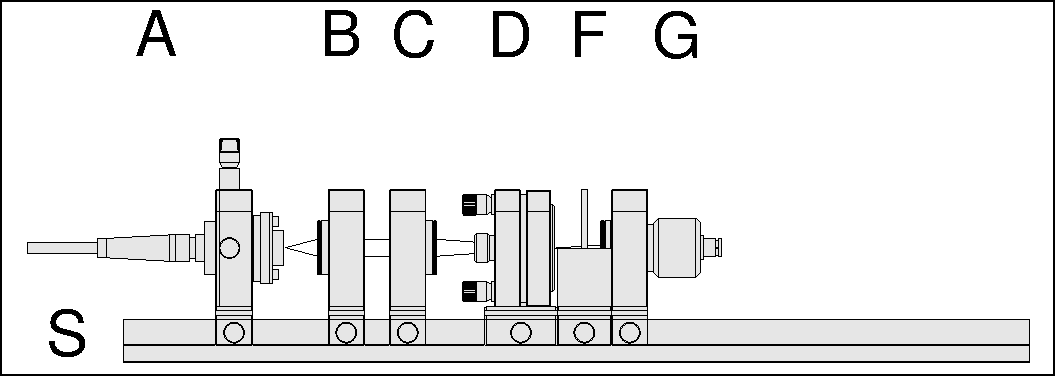
\includegraphics[width=0.9\textwidth]{setup_tau.pdf}
	\caption[Setup for measuring the lifetime of the $^4\mathrm{F}_{3/2}$ state]{Setup for measuring the lifetime of the $^4\mathrm{F}_{3/2}$ state. In addition to previous setups, the collimated beam is focused (C) on the Nd:YAG rod (D), and passes through a RG 1000 filter (F) which absorbs the remaining part of the pump beam. Both the modulated signal of the diode laser and the photo detector (G) are displayed in an oscilloscope (see figure \ref{fig:tau_osci}). \cite{lit:manual}}
	\label{fig:setup_tau}
\end{figure}

\begin{figure}[h]
	\centering
	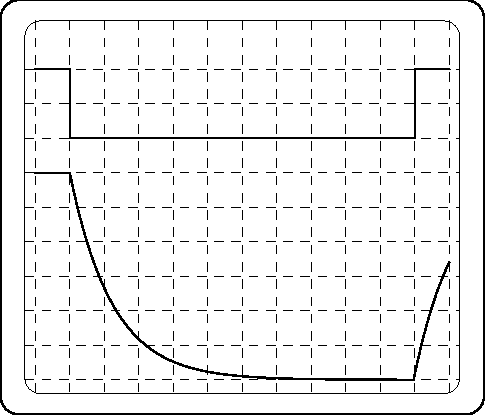
\includegraphics[width=0.5\textwidth]{tau_osci.pdf}
	\caption[Mean lifetime: Oscilloscope]{Oscilloscope display with modulation signal and photo detector signal. \cite{lit:manual}}
	\label{fig:tau_osci}
\end{figure}

We keep the current $I$ and the temperature $T$ constant. The mean lifetime $\tau_{1/2}$ is defined as the time in an exponential decay after which 1/e of an initial value is left. In this case we consider the intensity of the spontaneous emission. For three different modulation frequencies, we receive the periods $T_\text{decay}$ and the mean lifetimes $\tau_{1/2}$ entered in table \ref{tab:tau}.

\begin{table}[h]
	\centering
	\caption{Results for the mean lifetimes $\tau_{1/2}$.}
	\begin{tabular}{|c|c|}
	\hline
	$T_\text{decay}~(\milli\second)$ & $\tau_{1/2}~(\milli\second)$\\
	\hline
	2,925	& 0,2\\
	2	& 0,22\\
	2,5 &	0,21\\
	\hline
	\end{tabular}
	\label{tab:tau}
\end{table}

This gives us the average of $\tau_\text{1/2,mean}=(0,21\pm 0,01)\milli\second$, which is slightly lower than the estimated value of $0,25\milli\second$ given from \cite{lit:manual}. A reason for this deviation is unknown, reading errors and misadjustment of the focusing unit are probable.
\subsubsection{Nd:YAG laser power $P$ for various pump laser wavelengths}
For a given pump laser power $P_\text{diode}$, we inspect the wavelength dependence of the Nd:YAG laser output. Since the wavelength depends on the injection current $I$ and the temperature $T$ - as shown in section \ref{sec:diode_laser_lambda}, we can use its results to determine the corresponding wavelengths at given $P_\text{diode}=50,100,150\milli\watt$.
This is done as follows:
We take the measurements plotted in figure \ref{fig:measurement_P}. As we concluded those slopes are linear beyond the threshold current, we use the curve fit for $T=15\celsius$ and $T=35\celsius$ to the model function
\begin{align}
P_\text{diode}=m_1\cdot I+P_0(T),
\label{eq:P_linear}
\end{align}
while $P_0(T)$ is the temperature-dependent offset. Since $P_\text{diode}$ is kept constant, we can solve equation \eqref{eq:P_linear} using \eqref{eq:avg_slope1} for 
\begin{align}
I=\tfrac{P_\text{diode}-P_0(T)}{m}.
\end{align}
We can associate the currents $I_\text{min}$ to $T=15\celsius$ and $I_\text{max}$ to $T=35\celsius$ at a given $P_\text{diode}$. Those values are given in table \ref{tab:current_P}.

\begin{table}[h]
	\centering
	\caption{Currents for given $T$ and $P_\text{diode}$}
	\begin{tabular}{|c|c c|}
	\hline
	$P_\text{diode}~(\milli\watt)$ & $I_\text{min}~(\milli\ampere)$ & $I_\text{max}~(\milli\ampere)$\\
	\hline
	50 & 292.75 & 312.71\\
	100 & 385.18 & 406.69\\
	150 & 477.60 & 500.66\\
	\hline
	\end{tabular}
	\label{tab:current_P}
\end{table}

This results in the equation
\begin{align}
I_{P_\text{diode}}(T)=I_\text{min}+\tfrac{T-15\celsius}{20\celsius}\left(I_\text{max}-I_\text{min}\right),
\label{eq:current_P}
\end{align}
which can be inserted into equation \eqref{eq:lambda1}. We receive
\begin{align}
\lambda_{P_\text{diode}}(T)=\lambda_0+c_1\cdot \left(I_\text{min}+\tfrac{T-15\celsius}{20\celsius}(I_\text{max}-I_\text{min})\right)+c_2\cdot T,
\label{eq:lambda2}
\end{align}
and can compute the wavelength $\lambda_{P_\text{diode}}$ associated with $I$ and $T$ at a given $P_\text{diode}$.
For the measurement, we add a laser mirror in the existing setup and adjust the distance and angle to the Nd:YAG rod (see figure \ref{fig:setup_Nd:YAG}).

\begin{figure}[h]
	\centering
	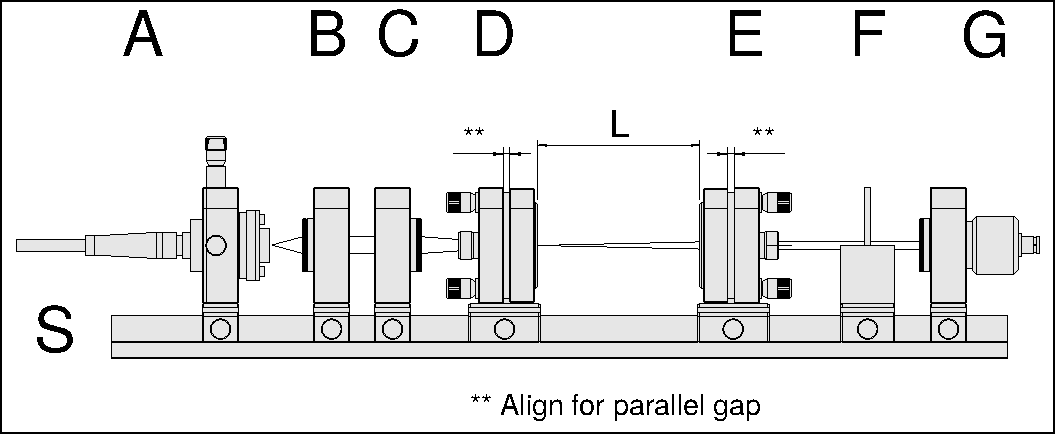
\includegraphics[width=0.9\textwidth]{setup_Nd_YAG.pdf}
	\caption[Setup of the Nd:YAG laser]{Setup of the Nd:YAG laser. A second resonator (E) is added and adjusted to maximize the output power. \cite{lit:manual}}
	\label{fig:setup_Nd:YAG}
\end{figure}

We figured the output power is maximized in multimode operation. This is achieved by adjusting the pump laser, the Nd:YAG rod and the second resonator such that both longitudinal and transversal modes are pumped and emitted.
The photo detector is set to detect the output power $P$ at the output wavelength of $\lambda=1064\nano\metre$. The measurements are conducted by determining the power while increasing the temperature and the current coarsely to keep the diode power mostly constant.
The results are depicted in figure \ref{fig:lambda2}.

\begin{figure}[h]
	\centering
	% This file was created by matlab2tikz.
% Minimal pgfplots version: 1.3
%
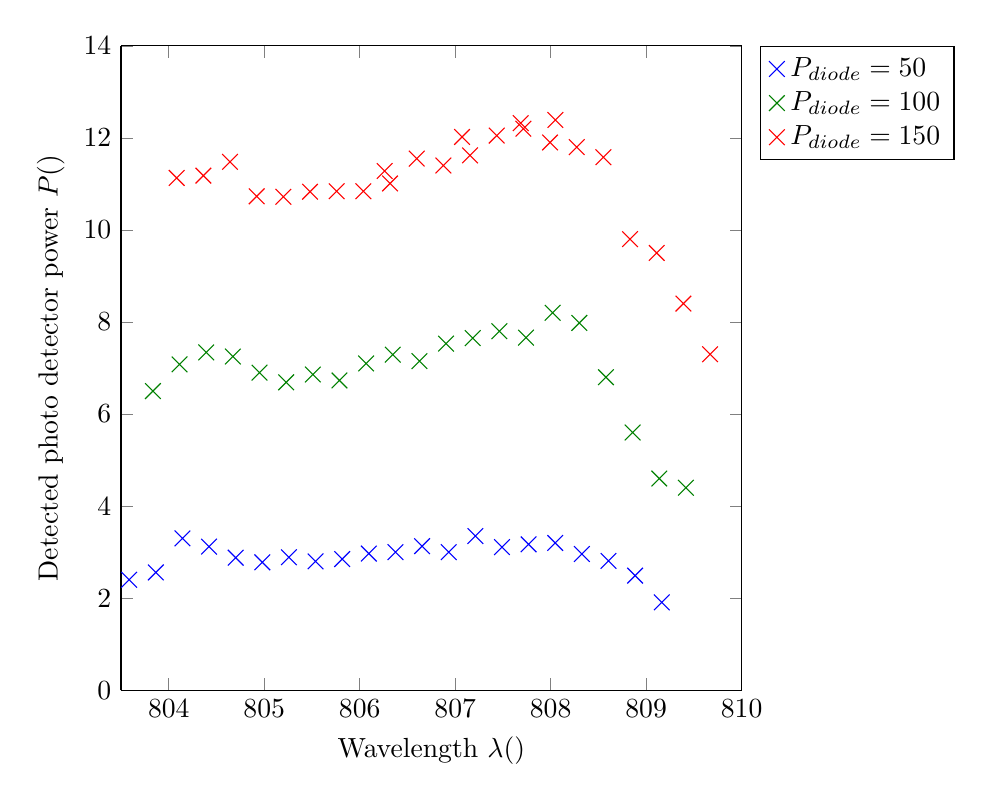
\begin{tikzpicture}

\begin{axis}[%
width=0.65\textwidth,
height=0.675\textwidth,
at={(0\textwidth,0\textwidth)},
scale only axis,
unbounded coords=jump,
separate axis lines,
every outer x axis line/.append style={black},
every x tick label/.append style={font=\color{black}},
xmin=803.5,
xmax=810,
xlabel={Wavelength $\lambda(\nano\metre)$},
every outer y axis line/.append style={black},
every y tick label/.append style={font=\color{black}},
ymin=0,
ymax=14,
ylabel={Detected photo detector power $P(\milli\watt)$},
legend style={at={(1.03,1)},anchor=north west,legend cell align=left,align=left,draw=black}
]
\addplot [color=blue,mark size=4.0pt,only marks,mark=x,mark options={solid}]
  table[row sep=crcr]{%
803.585287660711	2.4\\
803.864208588817	2.56\\
804.143129516922	3.3\\
804.422050445027	3.12\\
804.700971373132	2.88\\
804.979892301237	2.78\\
805.258813229342	2.89\\
805.537734157448	2.8\\
805.760870899932	nan\\
805.816655085553	2.85\\
806.095576013658	2.97\\
806.374496941763	3\\
806.569741591437	nan\\
806.653417869868	3.13\\
806.932338797973	3\\
807.183367633268	nan\\
807.211259726078	3.35\\
807.490180654184	3.11\\
807.545964839805	nan\\
807.769101582289	3.17\\
808.048022510394	3.2\\
808.326943438499	2.96\\
808.605864366604	2.81\\
808.884785294709	2.49\\
809.163706222815	1.91\\
};
\addlegendentry{$P_\text{diode}=50\milli\watt$};

\addplot [color=black!50!green,mark size=4.0pt,only marks,mark=x,mark options={solid}]
  table[row sep=crcr]{%
803.834100802076	6.5\\
804.113230076533	7.08\\
804.392359350989	7.34\\
804.671488625445	7.25\\
804.950617899901	6.9\\
805.229747174358	6.69\\
805.508876448814	6.86\\
805.78800572327	6.73\\
806.011309142835	nan\\
806.067134997726	7.1\\
806.346264272183	7.29\\
806.625393546639	7.15\\
806.820784038758	nan\\
806.904522821095	7.53\\
807.183652095551	7.65\\
807.434868442562	nan\\
807.462781370007	7.8\\
807.741910644464	7.66\\
807.797736499355	nan\\
808.02103991892	8.2\\
808.300169193376	7.98\\
808.579298467832	6.8\\
808.858427742289	5.6\\
809.137557016745	4.6\\
809.416686291201	4.4\\
};
\addlegendentry{$P_\text{diode}=100\milli\watt$};

\addplot [color=red,mark size=4.0pt,only marks,mark=x,mark options={solid}]
  table[row sep=crcr]{%
804.082913943441	11.13\\
804.362251564248	11.18\\
804.641589185056	11.48\\
804.920926805863	10.73\\
805.200264426671	10.72\\
805.479602047478	10.83\\
805.758939668285	10.84\\
806.038277289093	10.84\\
806.261747385738	11.28\\
806.3176149099	11.01\\
806.596952530707	11.55\\
806.876290151515	11.4\\
807.07182648608	12.02\\
807.155627772322	11.62\\
807.434965393129	12.05\\
807.686369251856	12.32\\
807.714303013937	12.2\\
807.993640634744	11.9\\
808.049508158905	12.39\\
808.272978255551	11.8\\
808.552315876359	11.58\\
808.831653497166	9.8\\
809.110991117973	9.5\\
809.390328738781	8.4\\
809.669666359588	7.3\\
};
\addlegendentry{$P_\text{diode}=150\milli\watt$};

\end{axis}
\end{tikzpicture}%
	\caption{Nd:YAG laser output power $P_{1064}(\lambda)$.}
	\label{fig:lambda2}
\end{figure}

We can see the maximal Nd:YAG laser output power $P_{1064}(\lambda)$ is at $\lambda_\text{max}\approx 808\nano\metre$, since there is a global maximum at $P_\text{diode}=100\milli\watt$ and $150\milli\watt$ whereas at $50\milli\watt$ it is a local maximum (most likelys due to measurement errors).
The absorption maximum of the Nd:YAG crystal is located at $808,4\nano\metre$. Inserting $\lambda_\text{max}$ into equation \eqref{eq:lambda2} and solving for $T$ yields $T\approx 29\celsius$, which gives us the parameter for the optimal laser mode.
\subsubsection{Nd:YAG laser power $P$: Dependence on $P_\text{diode}$}
Since the optimal temperature has been found before, we inspect the dependence of the Nd:YAG laser output power $P_{1064}$ on the power of the diode laser $P_\text{diode}$ for given temperature $T_\text{max}=29\celsius$. The experimental setup stays unchanged. Now we increase the injection current $I$ and measure the output power $P_{1064}$. Since the diode laser power $P_\text{diode}$ is linear to $I$ - as shown in figure \ref{fig:lambda1} - we can plot $P_{1064}$ against $P_\text{diode}$, see figure \ref{fig:P1064}.

\begin{figure}[h]
	\centering
	% This file was created by matlab2tikz.
% Minimal pgfplots version: 1.3
%
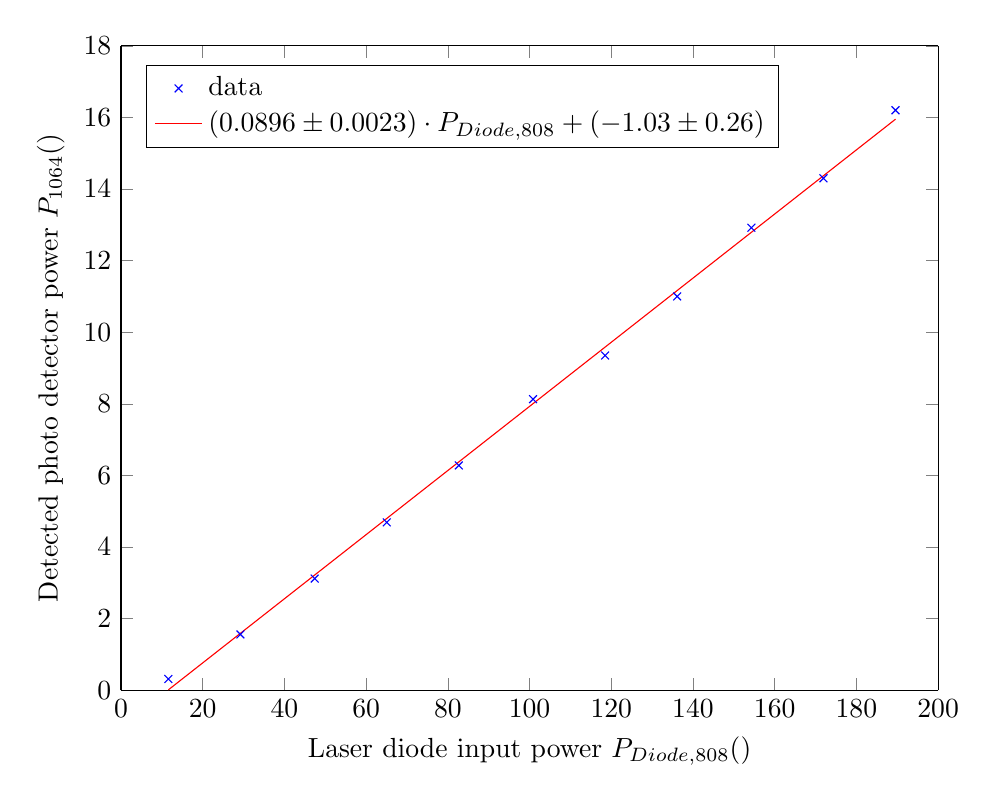
\begin{tikzpicture}

\begin{axis}[%
width=0.855828\textwidth,
height=0.675\textwidth,
at={(0\textwidth,0\textwidth)},
scale only axis,
separate axis lines,
every outer x axis line/.append style={black},
every x tick label/.append style={font=\color{black}},
xmin=0,
xmax=200,
xlabel={Laser diode input power $P_\text{Diode,808}(\milli\watt)$},
every outer y axis line/.append style={black},
every y tick label/.append style={font=\color{black}},
ymin=0,
ymax=18,
ylabel={Detected photo detector power $P_{1064}(\milli\watt)$},
legend style={at={(0.03,0.97)},anchor=north west,legend cell align=left,align=left,draw=black}
]
\addplot [color=blue,only marks,mark=x,mark options={solid}]
  table[row sep=crcr]{%
11.5874345238094	0.316\\
29.2253452380952	1.56\\
47.397738095238	3.12\\
65.0356488095237	4.69\\
82.6735595238095	6.28\\
100.845952380952	8.13\\
118.483863095238	9.35\\
136.121773809524	11\\
154.294166666667	12.92\\
171.932077380952	14.3\\
189.569988095238	16.2\\
};
\addlegendentry{data};

\addplot [color=red,solid]
  table[row sep=crcr]{%
11.5874345238094	0.0118188344330659\\
11.7654170773809	0.0277577791190842\\
11.9433996309523	0.0436967238051025\\
12.1213821845237	0.059635668491121\\
12.2993647380952	0.0755746131771393\\
12.4773472916666	0.0915135578631576\\
12.655329845238	0.107452502549176\\
12.8333123988094	0.123391447235194\\
13.0112949523809	0.139330391921213\\
13.1892775059523	0.155269336607231\\
13.3672600595237	0.171208281293249\\
13.5452426130952	0.187147225979268\\
13.7232251666666	0.203086170665286\\
13.901207720238	0.219025115351305\\
14.0791902738094	0.234964060037323\\
14.2571728273809	0.250903004723341\\
14.4351553809523	0.26684194940936\\
14.6131379345237	0.282780894095378\\
14.7911204880952	0.298719838781397\\
14.9691030416666	0.314658783467415\\
15.147085595238	0.330597728153433\\
15.3250681488095	0.346536672839452\\
15.5030507023809	0.36247561752547\\
15.6810332559523	0.378414562211488\\
15.8590158095237	0.394353506897507\\
16.0369983630952	0.410292451583525\\
16.2149809166666	0.426231396269543\\
16.392963470238	0.442170340955562\\
16.5709460238094	0.45810928564158\\
16.7489285773809	0.474048230327599\\
16.9269111309523	0.489987175013617\\
17.1048936845237	0.505926119699635\\
17.2828762380952	0.521865064385654\\
17.4608587916666	0.537804009071672\\
17.638841345238	0.55374295375769\\
17.8168238988094	0.569681898443709\\
17.9948064523809	0.585620843129727\\
18.1727890059523	0.601559787815745\\
18.3507715595237	0.617498732501764\\
18.5287541130952	0.633437677187782\\
18.7067366666666	0.649376621873801\\
18.884719220238	0.665315566559819\\
19.0627017738095	0.681254511245837\\
19.2406843273809	0.697193455931856\\
19.4186668809523	0.713132400617874\\
19.5966494345237	0.729071345303892\\
19.7746319880952	0.745010289989911\\
19.9526145416666	0.760949234675929\\
20.130597095238	0.776888179361948\\
20.3085796488094	0.792827124047966\\
20.4865622023809	0.808766068733985\\
20.6645447559523	0.824705013420002\\
20.8425273095237	0.840643958106021\\
21.0205098630952	0.856582902792039\\
21.1984924166666	0.872521847478058\\
21.376474970238	0.888460792164076\\
21.5544575238095	0.904399736850094\\
21.7324400773809	0.920338681536113\\
21.9104226309523	0.936277626222131\\
22.0884051845237	0.95221657090815\\
22.2663877380952	0.968155515594168\\
22.4443702916666	0.984094460280186\\
22.622352845238	1.0000334049662\\
22.8003353988095	1.01597234965222\\
22.9783179523809	1.03191129433824\\
23.1563005059523	1.04785023902426\\
23.3342830595237	1.06378918371028\\
23.5122656130952	1.0797281283963\\
23.6902481666666	1.09566707308231\\
23.868230720238	1.11160601776833\\
24.0462132738095	1.12754496245435\\
24.2241958273809	1.14348390714037\\
24.4021783809523	1.15942285182639\\
24.5801609345237	1.17536179651241\\
24.7581434880952	1.19130074119843\\
24.9361260416666	1.20723968588444\\
25.114108595238	1.22317863057046\\
25.2920911488095	1.23911757525648\\
25.4700737023809	1.2550565199425\\
25.6480562559523	1.27099546462852\\
25.8260388095237	1.28693440931454\\
26.0040213630952	1.30287335400055\\
26.1820039166666	1.31881229868657\\
26.359986470238	1.33475124337259\\
26.5379690238095	1.35069018805861\\
26.7159515773809	1.36662913274463\\
26.8939341309523	1.38256807743065\\
27.0719166845237	1.39850702211666\\
27.2498992380952	1.41444596680268\\
27.4278817916666	1.4303849114887\\
27.605864345238	1.44632385617472\\
27.7838468988095	1.46226280086074\\
27.9618294523809	1.47820174554676\\
28.1398120059523	1.49414069023277\\
28.3177945595237	1.51007963491879\\
28.4957771130952	1.52601857960481\\
28.6737596666666	1.54195752429083\\
28.851742220238	1.55789646897685\\
29.0297247738095	1.57383541366287\\
29.2077073273809	1.58977435834888\\
29.2253452380952	1.59135389340786\\
29.3856898809523	1.6057133030349\\
29.5636724345237	1.62165224772092\\
29.7416549880952	1.63759119240694\\
29.9196375416666	1.65353013709296\\
30.097620095238	1.66946908177898\\
30.2756026488095	1.68540802646499\\
30.4535852023809	1.70134697115101\\
30.6315677559523	1.71728591583703\\
30.8095503095237	1.73322486052305\\
30.9875328630952	1.74916380520907\\
31.1655154166666	1.76510274989509\\
31.343497970238	1.78104169458111\\
31.5214805238095	1.79698063926712\\
31.6994630773809	1.81291958395314\\
31.8774456309523	1.82885852863916\\
32.0554281845237	1.84479747332518\\
32.2334107380952	1.8607364180112\\
32.4113932916666	1.87667536269722\\
32.589375845238	1.89261430738323\\
32.7673583988094	1.90855325206925\\
32.9453409523809	1.92449219675527\\
33.1233235059523	1.94043114144129\\
33.3013060595237	1.95637008612731\\
33.4792886130952	1.97230903081333\\
33.6572711666666	1.98824797549934\\
33.835253720238	2.00418692018536\\
34.0132362738095	2.02012586487138\\
34.1912188273809	2.0360648095574\\
34.3692013809523	2.05200375424342\\
34.5471839345237	2.06794269892944\\
34.7251664880952	2.08388164361545\\
34.9031490416666	2.09982058830147\\
35.081131595238	2.11575953298749\\
35.2591141488095	2.13169847767351\\
35.4370967023809	2.14763742235953\\
35.6150792559523	2.16357636704555\\
35.7930618095237	2.17951531173156\\
35.9710443630952	2.19545425641758\\
36.1490269166666	2.2113932011036\\
36.327009470238	2.22733214578962\\
36.5049920238095	2.24327109047564\\
36.6829745773809	2.25921003516166\\
36.8609571309523	2.27514897984767\\
37.0389396845237	2.29108792453369\\
37.2169222380952	2.30702686921971\\
37.3949047916666	2.32296581390573\\
37.572887345238	2.33890475859175\\
37.7508698988095	2.35484370327777\\
37.9288524523809	2.37078264796378\\
38.1068350059523	2.3867215926498\\
38.2848175595237	2.40266053733582\\
38.4628001130952	2.41859948202184\\
38.6407826666666	2.43453842670786\\
38.818765220238	2.45047737139388\\
38.9967477738095	2.46641631607989\\
39.1747303273809	2.48235526076591\\
39.3527128809523	2.49829420545193\\
39.5306954345237	2.51423315013795\\
39.7086779880952	2.53017209482397\\
39.8866605416666	2.54611103950999\\
40.064643095238	2.562049984196\\
40.2426256488095	2.57798892888202\\
40.4206082023809	2.59392787356804\\
40.5985907559523	2.60986681825406\\
40.7765733095237	2.62580576294008\\
40.9545558630952	2.6417447076261\\
41.1325384166666	2.65768365231212\\
41.310520970238	2.67362259699813\\
41.4885035238095	2.68956154168415\\
41.6664860773809	2.70550048637017\\
41.8444686309523	2.72143943105619\\
42.0224511845237	2.73737837574221\\
42.2004337380952	2.75331732042823\\
42.3784162916666	2.76925626511424\\
42.556398845238	2.78519520980026\\
42.7343813988094	2.80113415448628\\
42.9123639523809	2.8170730991723\\
43.0903465059523	2.83301204385832\\
43.2683290595237	2.84895098854434\\
43.4463116130952	2.86488993323035\\
43.6242941666666	2.88082887791637\\
43.802276720238	2.89676782260239\\
43.9802592738095	2.91270676728841\\
44.1582418273809	2.92864571197443\\
44.3362243809523	2.94458465666045\\
44.5142069345237	2.96052360134646\\
44.6921894880952	2.97646254603248\\
44.8701720416666	2.9924014907185\\
45.048154595238	3.00834043540452\\
45.2261371488095	3.02427938009054\\
45.4041197023809	3.04021832477656\\
45.5821022559523	3.05615726946257\\
45.7600848095237	3.07209621414859\\
45.9380673630952	3.08803515883461\\
46.1160499166666	3.10397410352063\\
46.294032470238	3.11991304820665\\
46.4720150238095	3.13585199289267\\
46.6499975773809	3.15179093757869\\
46.8279801309523	3.1677298822647\\
47.0059626845237	3.18366882695072\\
47.1839452380952	3.19960777163674\\
47.3619277916666	3.21554671632276\\
47.397738095238	3.21875365113946\\
47.539910345238	3.23148566100878\\
47.7178928988095	3.2474246056948\\
47.8958754523809	3.26336355038081\\
48.0738580059523	3.27930249506683\\
48.2518405595237	3.29524143975285\\
48.4298231130952	3.31118038443887\\
48.6078056666666	3.32711932912489\\
48.785788220238	3.34305827381091\\
48.9637707738095	3.35899721849692\\
49.1417533273809	3.37493616318294\\
49.3197358809523	3.39087510786896\\
49.4977184345237	3.40681405255498\\
49.6757009880952	3.422752997241\\
49.8536835416666	3.43869194192702\\
50.031666095238	3.45463088661303\\
50.2096486488095	3.47056983129905\\
50.3876312023809	3.48650877598507\\
50.5656137559523	3.50244772067109\\
50.7435963095237	3.51838666535711\\
50.9215788630952	3.53432561004313\\
51.0995614166666	3.55026455472914\\
51.277543970238	3.56620349941516\\
51.4555265238095	3.58214244410118\\
51.6335090773809	3.5980813887872\\
51.8114916309523	3.61402033347322\\
51.9894741845237	3.62995927815924\\
52.1674567380952	3.64589822284525\\
52.3454392916666	3.66183716753127\\
52.523421845238	3.67777611221729\\
52.7014043988095	3.69371505690331\\
52.8793869523809	3.70965400158933\\
53.0573695059523	3.72559294627535\\
53.2353520595237	3.74153189096136\\
53.4133346130952	3.75747083564738\\
53.5913171666666	3.7734097803334\\
53.769299720238	3.78934872501942\\
53.9472822738094	3.80528766970544\\
54.1252648273809	3.82122661439146\\
54.3032473809523	3.83716555907747\\
54.4812299345237	3.85310450376349\\
54.6592124880952	3.86904344844951\\
54.8371950416666	3.88498239313553\\
55.015177595238	3.90092133782155\\
55.1931601488095	3.91686028250757\\
55.3711427023809	3.93279922719359\\
55.5491252559523	3.9487381718796\\
55.7271078095237	3.96467711656562\\
55.9050903630952	3.98061606125164\\
56.0830729166666	3.99655500593766\\
56.261055470238	4.01249395062368\\
56.4390380238095	4.0284328953097\\
56.6170205773809	4.04437183999571\\
56.7950031309523	4.06031078468173\\
56.9729856845237	4.07624972936775\\
57.1509682380952	4.09218867405377\\
57.3289507916666	4.10812761873979\\
57.506933345238	4.12406656342581\\
57.6849158988095	4.14000550811182\\
57.8628984523809	4.15594445279784\\
58.0408810059523	4.17188339748386\\
58.2188635595237	4.18782234216988\\
58.3968461130952	4.2037612868559\\
58.5748286666666	4.21970023154192\\
58.752811220238	4.23563917622793\\
58.9307937738095	4.25157812091395\\
59.1087763273809	4.26751706559997\\
59.2867588809523	4.28345601028599\\
59.4647414345237	4.29939495497201\\
59.6427239880952	4.31533389965803\\
59.8207065416666	4.33127284434404\\
59.998689095238	4.34721178903006\\
60.1766716488095	4.36315073371608\\
60.3546542023809	4.3790896784021\\
60.5326367559523	4.39502862308812\\
60.7106193095237	4.41096756777414\\
60.8886018630952	4.42690651246015\\
61.0665844166666	4.44284545714617\\
61.244566970238	4.45878440183219\\
61.4225495238095	4.47472334651821\\
61.6005320773809	4.49066229120423\\
61.7785146309523	4.50660123589025\\
61.9564971845237	4.52254018057626\\
62.1344797380952	4.53847912526228\\
62.3124622916666	4.5544180699483\\
62.490444845238	4.57035701463432\\
62.6684273988095	4.58629595932034\\
62.8464099523809	4.60223490400636\\
63.0243925059523	4.61817384869237\\
63.2023750595237	4.63411279337839\\
63.3803576130952	4.65005173806441\\
63.5583401666666	4.66599068275043\\
63.736322720238	4.68192962743645\\
63.9143052738095	4.69786857212247\\
64.0922878273809	4.71380751680849\\
64.2702703809523	4.7297464614945\\
64.4482529345237	4.74568540618052\\
64.6262354880952	4.76162435086654\\
64.8042180416666	4.77756329555256\\
64.982200595238	4.79350224023858\\
65.0356488095237	4.79828871011426\\
65.1601831488095	4.8094411849246\\
65.3381657023809	4.82538012961061\\
65.5161482559523	4.84131907429663\\
65.6941308095237	4.85725801898265\\
65.8721133630952	4.87319696366867\\
66.0500959166666	4.88913590835469\\
66.228078470238	4.9050748530407\\
66.4060610238095	4.92101379772672\\
66.5840435773809	4.93695274241274\\
66.7620261309523	4.95289168709876\\
66.9400086845237	4.96883063178478\\
67.1179912380952	4.9847695764708\\
67.2959737916666	5.00070852115682\\
67.473956345238	5.01664746584283\\
67.6519388988094	5.03258641052885\\
67.8299214523809	5.04852535521487\\
68.0079040059523	5.06446429990089\\
68.1858865595237	5.08040324458691\\
68.3638691130952	5.09634218927293\\
68.5418516666666	5.11228113395894\\
68.719834220238	5.12822007864496\\
68.8978167738095	5.14415902333098\\
69.0757993273809	5.160097968017\\
69.2537818809523	5.17603691270302\\
69.4317644345237	5.19197585738904\\
69.6097469880952	5.20791480207505\\
69.7877295416666	5.22385374676107\\
69.965712095238	5.23979269144709\\
70.1436946488095	5.25573163613311\\
70.3216772023809	5.27167058081913\\
70.4996597559523	5.28760952550515\\
70.6776423095237	5.30354847019117\\
70.8556248630952	5.31948741487718\\
71.0336074166666	5.3354263595632\\
71.211589970238	5.35136530424922\\
71.3895725238094	5.36730424893524\\
71.5675550773809	5.38324319362126\\
71.7455376309523	5.39918213830727\\
71.9235201845237	5.41512108299329\\
72.1015027380952	5.43106002767931\\
72.2794852916666	5.44699897236533\\
72.457467845238	5.46293791705135\\
72.6354503988095	5.47887686173737\\
72.8134329523809	5.49481580642339\\
72.9914155059523	5.5107547511094\\
73.1693980595237	5.52669369579542\\
73.3473806130952	5.54263264048144\\
73.5253631666666	5.55857158516746\\
73.703345720238	5.57451052985348\\
73.8813282738095	5.5904494745395\\
74.0593108273809	5.60638841922551\\
74.2372933809523	5.62232736391153\\
74.4152759345237	5.63826630859755\\
74.5932584880952	5.65420525328357\\
74.7712410416666	5.67014419796959\\
74.949223595238	5.68608314265561\\
75.1272061488094	5.70202208734162\\
75.3051887023809	5.71796103202764\\
75.4831712559523	5.73389997671366\\
75.6611538095237	5.74983892139968\\
75.8391363630952	5.7657778660857\\
76.0171189166666	5.78171681077172\\
76.195101470238	5.79765575545773\\
76.3730840238095	5.81359470014375\\
76.5510665773809	5.82953364482977\\
76.7290491309523	5.84547258951579\\
76.9070316845237	5.86141153420181\\
77.0850142380952	5.87735047888783\\
77.2629967916666	5.89328942357384\\
77.440979345238	5.90922836825986\\
77.6189618988095	5.92516731294588\\
77.7969444523809	5.9411062576319\\
77.9749270059523	5.95704520231792\\
78.1529095595237	5.97298414700394\\
78.3308921130952	5.98892309168996\\
78.5088746666666	6.00486203637597\\
78.686857220238	6.02080098106199\\
78.8648397738095	6.03673992574801\\
79.0428223273809	6.05267887043403\\
79.2208048809523	6.06861781512005\\
79.3987874345237	6.08455675980606\\
79.5767699880952	6.10049570449208\\
79.7547525416666	6.1164346491781\\
79.932735095238	6.13237359386412\\
80.1107176488095	6.14831253855014\\
80.2887002023809	6.16425148323616\\
80.4666827559523	6.18019042792217\\
80.6446653095237	6.19612937260819\\
80.8226478630952	6.21206831729421\\
81.0006304166666	6.22800726198023\\
81.178612970238	6.24394620666625\\
81.3565955238095	6.25988515135227\\
81.5345780773809	6.27582409603829\\
81.7125606309523	6.2917630407243\\
81.8905431845237	6.30770198541032\\
82.0685257380952	6.32364093009634\\
82.2465082916666	6.33957987478236\\
82.424490845238	6.35551881946838\\
82.6024733988095	6.3714577641544\\
82.6735595238095	6.37782376908905\\
82.7804559523809	6.38739670884041\\
82.9584385059523	6.40333565352643\\
83.1364210595237	6.41927459821245\\
83.3144036130952	6.43521354289847\\
83.4923861666666	6.45115248758449\\
83.670368720238	6.46709143227051\\
83.8483512738095	6.48303037695652\\
84.0263338273809	6.49896932164254\\
84.2043163809523	6.51490826632856\\
84.3822989345237	6.53084721101458\\
84.5602814880952	6.5467861557006\\
84.7382640416666	6.56272510038662\\
84.916246595238	6.57866404507263\\
85.0942291488095	6.59460298975865\\
85.2722117023809	6.61054193444467\\
85.4501942559523	6.62648087913069\\
85.6281768095237	6.64241982381671\\
85.8061593630952	6.65835876850273\\
85.9841419166666	6.67429771318874\\
86.162124470238	6.69023665787476\\
86.3401070238095	6.70617560256078\\
86.5180895773809	6.7221145472468\\
86.6960721309523	6.73805349193282\\
86.8740546845237	6.75399243661884\\
87.0520372380952	6.76993138130485\\
87.2300197916666	6.78587032599087\\
87.408002345238	6.80180927067689\\
87.5859848988095	6.81774821536291\\
87.7639674523809	6.83368716004893\\
87.9419500059523	6.84962610473495\\
88.1199325595237	6.86556504942097\\
88.2979151130952	6.88150399410698\\
88.4758976666666	6.897442938793\\
88.653880220238	6.91338188347902\\
88.8318627738095	6.92932082816504\\
89.0098453273809	6.94525977285106\\
89.1878278809523	6.96119871753708\\
89.3658104345237	6.97713766222309\\
89.5437929880952	6.99307660690911\\
89.7217755416666	7.00901555159513\\
89.899758095238	7.02495449628115\\
90.0777406488095	7.04089344096717\\
90.2557232023809	7.05683238565318\\
90.4337057559523	7.0727713303392\\
90.6116883095237	7.08871027502522\\
90.7896708630952	7.10464921971124\\
90.9676534166666	7.12058816439726\\
91.145635970238	7.13652710908328\\
91.3236185238095	7.1524660537693\\
91.5016010773809	7.16840499845531\\
91.6795836309523	7.18434394314133\\
91.8575661845237	7.20028288782735\\
92.0355487380952	7.21622183251337\\
92.2135312916666	7.23216077719939\\
92.391513845238	7.2480997218854\\
92.5694963988095	7.26403866657142\\
92.7474789523809	7.27997761125744\\
92.9254615059523	7.29591655594346\\
93.1034440595237	7.31185550062948\\
93.2814266130952	7.3277944453155\\
93.4594091666666	7.34373339000152\\
93.637391720238	7.35967233468753\\
93.8153742738095	7.37561127937355\\
93.9933568273809	7.39155022405957\\
94.1713393809523	7.40748916874559\\
94.3493219345237	7.42342811343161\\
94.5273044880952	7.43936705811763\\
94.7052870416666	7.45530600280364\\
94.883269595238	7.47124494748966\\
95.0612521488095	7.48718389217568\\
95.2392347023809	7.5031228368617\\
95.4172172559523	7.51906178154772\\
95.5951998095237	7.53500072623374\\
95.7731823630952	7.55093967091975\\
95.9511649166666	7.56687861560577\\
96.129147470238	7.58281756029179\\
96.3071300238094	7.59875650497781\\
96.4851125773809	7.61469544966383\\
96.6630951309523	7.63063439434985\\
96.8410776845237	7.64657333903586\\
97.0190602380952	7.66251228372188\\
97.1970427916666	7.6784512284079\\
97.375025345238	7.69439017309392\\
97.5530078988095	7.71032911777994\\
97.7309904523809	7.72626806246596\\
97.9089730059523	7.74220700715198\\
98.0869555595237	7.75814595183799\\
98.2649381130952	7.77408489652401\\
98.4429206666666	7.79002384121003\\
98.620903220238	7.80596278589605\\
98.7988857738095	7.82190173058207\\
98.9768683273809	7.83784067526808\\
99.1548508809523	7.8537796199541\\
99.3328334345237	7.86971856464012\\
99.5108159880952	7.88565750932614\\
99.6887985416666	7.90159645401216\\
99.866781095238	7.91753539869818\\
100.044763648809	7.93347434338419\\
100.222746202381	7.94941328807021\\
100.400728755952	7.96535223275623\\
100.578711309524	7.98129117744225\\
100.756693863095	7.99723012212827\\
100.845952380952	8.00522352682066\\
100.934676416667	8.01316906681429\\
101.112658970238	8.02910801150031\\
101.290641523809	8.04504695618632\\
101.468624077381	8.06098590087234\\
101.646606630952	8.07692484555836\\
101.824589184524	8.09286379024438\\
102.002571738095	8.1088027349304\\
102.180554291667	8.12474167961641\\
102.358536845238	8.14068062430244\\
102.536519398809	8.15661956898845\\
102.714501952381	8.17255851367447\\
102.892484505952	8.18849745836049\\
103.070467059524	8.20443640304651\\
103.248449613095	8.22037534773253\\
103.426432166667	8.23631429241854\\
103.604414720238	8.25225323710456\\
103.782397273809	8.26819218179058\\
103.960379827381	8.2841311264766\\
104.138362380952	8.30007007116262\\
104.316344934524	8.31600901584864\\
104.494327488095	8.33194796053465\\
104.672310041667	8.34788690522067\\
104.850292595238	8.36382584990669\\
105.028275148809	8.37976479459271\\
105.206257702381	8.39570373927873\\
105.384240255952	8.41164268396475\\
105.562222809524	8.42758162865077\\
105.740205363095	8.44352057333678\\
105.918187916667	8.4594595180228\\
106.096170470238	8.47539846270882\\
106.274153023809	8.49133740739484\\
106.452135577381	8.50727635208086\\
106.630118130952	8.52321529676687\\
106.808100684524	8.53915424145289\\
106.986083238095	8.55509318613891\\
107.164065791667	8.57103213082493\\
107.342048345238	8.58697107551095\\
107.520030898809	8.60291002019697\\
107.698013452381	8.61884896488299\\
107.875996005952	8.634787909569\\
108.053978559524	8.65072685425502\\
108.231961113095	8.66666579894104\\
108.409943666667	8.68260474362706\\
108.587926220238	8.69854368831308\\
108.765908773809	8.7144826329991\\
108.943891327381	8.73042157768511\\
109.121873880952	8.74636052237113\\
109.299856434524	8.76229946705715\\
109.477838988095	8.77823841174317\\
109.655821541667	8.79417735642919\\
109.833804095238	8.8101163011152\\
110.011786648809	8.82605524580122\\
110.189769202381	8.84199419048724\\
110.367751755952	8.85793313517326\\
110.545734309524	8.87387207985928\\
110.723716863095	8.8898110245453\\
110.901699416667	8.90574996923132\\
111.079681970238	8.92168891391733\\
111.257664523809	8.93762785860335\\
111.435647077381	8.95356680328937\\
111.613629630952	8.96950574797539\\
111.791612184524	8.98544469266141\\
111.969594738095	9.00138363734743\\
112.147577291667	9.01732258203345\\
112.325559845238	9.03326152671946\\
112.503542398809	9.04920047140548\\
112.681524952381	9.0651394160915\\
112.859507505952	9.08107836077752\\
113.037490059524	9.09701730546354\\
113.215472613095	9.11295625014955\\
113.393455166667	9.12889519483557\\
113.571437720238	9.14483413952159\\
113.749420273809	9.16077308420761\\
113.927402827381	9.17671202889363\\
114.105385380952	9.19265097357965\\
114.283367934524	9.20858991826566\\
114.461350488095	9.22452886295168\\
114.639333041667	9.2404678076377\\
114.817315595238	9.25640675232372\\
114.995298148809	9.27234569700974\\
115.173280702381	9.28828464169576\\
115.351263255952	9.30422358638178\\
115.529245809524	9.32016253106779\\
115.707228363095	9.33610147575381\\
115.885210916667	9.35204042043983\\
116.063193470238	9.36797936512585\\
116.241176023809	9.38391830981187\\
116.419158577381	9.39985725449788\\
116.597141130952	9.4157961991839\\
116.775123684524	9.43173514386992\\
116.953106238095	9.44767408855594\\
117.131088791667	9.46361303324196\\
117.309071345238	9.47955197792798\\
117.487053898809	9.495490922614\\
117.665036452381	9.51142986730001\\
117.843019005952	9.52736881198603\\
118.021001559524	9.54330775667205\\
118.198984113095	9.55924670135807\\
118.376966666667	9.57518564604409\\
118.483863095238	9.58475858579545\\
118.554949220238	9.59112459073011\\
118.732931773809	9.60706353541612\\
118.910914327381	9.62300248010214\\
119.088896880952	9.63894142478816\\
119.266879434524	9.65488036947418\\
119.444861988095	9.6708193141602\\
119.622844541667	9.68675825884622\\
119.800827095238	9.70269720353224\\
119.978809648809	9.71863614821825\\
120.156792202381	9.73457509290427\\
120.334774755952	9.75051403759029\\
120.512757309524	9.76645298227631\\
120.690739863095	9.78239192696233\\
120.868722416667	9.79833087164834\\
121.046704970238	9.81426981633436\\
121.224687523809	9.83020876102038\\
121.402670077381	9.8461477057064\\
121.580652630952	9.86208665039242\\
121.758635184524	9.87802559507844\\
121.936617738095	9.89396453976446\\
122.114600291667	9.90990348445047\\
122.292582845238	9.92584242913649\\
122.470565398809	9.94178137382251\\
122.648547952381	9.95772031850853\\
122.826530505952	9.97365926319455\\
123.004513059524	9.98959820788057\\
123.182495613095	10.0055371525666\\
123.360478166667	10.0214760972526\\
123.538460720238	10.0374150419386\\
123.716443273809	10.0533539866246\\
123.894425827381	10.0692929313107\\
124.072408380952	10.0852318759967\\
124.250390934524	10.1011708206827\\
124.428373488095	10.1171097653687\\
124.606356041667	10.1330487100547\\
124.784338595238	10.1489876547407\\
124.962321148809	10.1649265994268\\
125.140303702381	10.1808655441128\\
125.318286255952	10.1968044887988\\
125.496268809524	10.2127434334848\\
125.674251363095	10.2286823781708\\
125.852233916667	10.2446213228569\\
126.030216470238	10.2605602675429\\
126.208199023809	10.2764992122289\\
126.386181577381	10.2924381569149\\
126.564164130952	10.3083771016009\\
126.742146684524	10.324316046287\\
126.920129238095	10.340254990973\\
127.098111791667	10.356193935659\\
127.276094345238	10.372132880345\\
127.454076898809	10.388071825031\\
127.632059452381	10.404010769717\\
127.810042005952	10.4199497144031\\
127.988024559524	10.4358886590891\\
128.166007113095	10.4518276037751\\
128.343989666667	10.4677665484611\\
128.521972220238	10.4837054931471\\
128.699954773809	10.4996444378332\\
128.877937327381	10.5155833825192\\
129.055919880952	10.5315223272052\\
129.233902434524	10.5474612718912\\
129.411884988095	10.5634002165772\\
129.589867541667	10.5793391612632\\
129.767850095238	10.5952781059493\\
129.945832648809	10.6112170506353\\
130.123815202381	10.6271559953213\\
130.301797755952	10.6430949400073\\
130.479780309524	10.6590338846933\\
130.657762863095	10.6749728293794\\
130.835745416667	10.6909117740654\\
131.013727970238	10.7068507187514\\
131.191710523809	10.7227896634374\\
131.369693077381	10.7387286081234\\
131.547675630952	10.7546675528094\\
131.725658184524	10.7706064974955\\
131.903640738095	10.7865454421815\\
132.081623291667	10.8024843868675\\
132.259605845238	10.8184233315535\\
132.437588398809	10.8343622762395\\
132.615570952381	10.8503012209256\\
132.793553505952	10.8662401656116\\
132.971536059524	10.8821791102976\\
133.149518613095	10.8981180549836\\
133.327501166667	10.9140569996696\\
133.505483720238	10.9299959443557\\
133.683466273809	10.9459348890417\\
133.861448827381	10.9618738337277\\
134.039431380952	10.9778127784137\\
134.217413934524	10.9937517230997\\
134.395396488095	11.0096906677857\\
134.573379041667	11.0256296124718\\
134.751361595238	11.0415685571578\\
134.929344148809	11.0575075018438\\
135.107326702381	11.0734464465298\\
135.285309255952	11.0893853912158\\
135.463291809524	11.1053243359019\\
135.641274363095	11.1212632805879\\
135.819256916667	11.1372022252739\\
135.997239470238	11.1531411699599\\
136.121773809524	11.1642936447702\\
136.175222023809	11.1690801146459\\
136.353204577381	11.1850190593319\\
136.531187130952	11.200958004018\\
136.709169684524	11.216896948704\\
136.887152238095	11.23283589339\\
137.065134791667	11.248774838076\\
137.243117345238	11.264713782762\\
137.421099898809	11.2806527274481\\
137.599082452381	11.2965916721341\\
137.777065005952	11.3125306168201\\
137.955047559524	11.3284695615061\\
138.133030113095	11.3444085061921\\
138.311012666667	11.3603474508781\\
138.488995220238	11.3762863955642\\
138.666977773809	11.3922253402502\\
138.844960327381	11.4081642849362\\
139.022942880952	11.4241032296222\\
139.200925434524	11.4400421743082\\
139.378907988095	11.4559811189943\\
139.556890541667	11.4719200636803\\
139.734873095238	11.4878590083663\\
139.912855648809	11.5037979530523\\
140.090838202381	11.5197368977383\\
140.268820755952	11.5356758424243\\
140.446803309524	11.5516147871104\\
140.624785863095	11.5675537317964\\
140.802768416667	11.5834926764824\\
140.980750970238	11.5994316211684\\
141.158733523809	11.6153705658544\\
141.336716077381	11.6313095105405\\
141.514698630952	11.6472484552265\\
141.692681184524	11.6631873999125\\
141.870663738095	11.6791263445985\\
142.048646291667	11.6950652892845\\
142.226628845238	11.7110042339706\\
142.404611398809	11.7269431786566\\
142.582593952381	11.7428821233426\\
142.760576505952	11.7588210680286\\
142.938559059524	11.7747600127146\\
143.116541613095	11.7906989574006\\
143.294524166667	11.8066379020867\\
143.472506720238	11.8225768467727\\
143.650489273809	11.8385157914587\\
143.828471827381	11.8544547361447\\
144.006454380952	11.8703936808307\\
144.184436934524	11.8863326255168\\
144.362419488095	11.9022715702028\\
144.540402041667	11.9182105148888\\
144.718384595238	11.9341494595748\\
144.896367148809	11.9500884042608\\
145.074349702381	11.9660273489468\\
145.252332255952	11.9819662936329\\
145.430314809524	11.9979052383189\\
145.608297363095	12.0138441830049\\
145.786279916667	12.0297831276909\\
145.964262470238	12.0457220723769\\
146.142245023809	12.061661017063\\
146.320227577381	12.077599961749\\
146.498210130952	12.093538906435\\
146.676192684524	12.109477851121\\
146.854175238095	12.125416795807\\
147.032157791667	12.141355740493\\
147.210140345238	12.1572946851791\\
147.388122898809	12.1732336298651\\
147.566105452381	12.1891725745511\\
147.744088005952	12.2051115192371\\
147.922070559524	12.2210504639231\\
148.100053113095	12.2369894086092\\
148.278035666667	12.2529283532952\\
148.456018220238	12.2688672979812\\
148.634000773809	12.2848062426672\\
148.811983327381	12.3007451873532\\
148.989965880952	12.3166841320392\\
149.167948434524	12.3326230767253\\
149.345930988095	12.3485620214113\\
149.523913541667	12.3645009660973\\
149.701896095238	12.3804399107833\\
149.879878648809	12.3963788554693\\
150.057861202381	12.4123178001554\\
150.235843755952	12.4282567448414\\
150.413826309524	12.4441956895274\\
150.591808863095	12.4601346342134\\
150.769791416667	12.4760735788994\\
150.947773970238	12.4920125235854\\
151.125756523809	12.5079514682715\\
151.303739077381	12.5238904129575\\
151.481721630952	12.5398293576435\\
151.659704184524	12.5557683023295\\
151.837686738095	12.5717072470155\\
152.015669291667	12.5876461917016\\
152.193651845238	12.6035851363876\\
152.371634398809	12.6195240810736\\
152.549616952381	12.6354630257596\\
152.727599505952	12.6514019704456\\
152.905582059524	12.6673409151317\\
153.083564613095	12.6832798598177\\
153.261547166667	12.6992188045037\\
153.439529720238	12.7151577491897\\
153.617512273809	12.7310966938757\\
153.795494827381	12.7470356385617\\
153.973477380952	12.7629745832478\\
154.151459934524	12.7789135279338\\
154.294166666667	12.7916934025019\\
154.329442488095	12.7948524726198\\
154.507425041667	12.8107914173058\\
154.685407595238	12.8267303619918\\
154.863390148809	12.8426693066779\\
155.041372702381	12.8586082513639\\
155.219355255952	12.8745471960499\\
155.397337809524	12.8904861407359\\
155.575320363095	12.9064250854219\\
155.753302916667	12.9223640301079\\
155.931285470238	12.938302974794\\
156.109268023809	12.95424191948\\
156.287250577381	12.970180864166\\
156.465233130952	12.986119808852\\
156.643215684524	13.002058753538\\
156.821198238095	13.0179976982241\\
156.999180791667	13.0339366429101\\
157.177163345238	13.0498755875961\\
157.355145898809	13.0658145322821\\
157.533128452381	13.0817534769681\\
157.711111005952	13.0976924216541\\
157.889093559524	13.1136313663402\\
158.067076113095	13.1295703110262\\
158.245058666667	13.1455092557122\\
158.423041220238	13.1614482003982\\
158.601023773809	13.1773871450842\\
158.779006327381	13.1933260897703\\
158.956988880952	13.2092650344563\\
159.134971434524	13.2252039791423\\
159.312953988095	13.2411429238283\\
159.490936541667	13.2570818685143\\
159.668919095238	13.2730208132004\\
159.846901648809	13.2889597578864\\
160.024884202381	13.3048987025724\\
160.202866755952	13.3208376472584\\
160.380849309524	13.3367765919444\\
160.558831863095	13.3527155366304\\
160.736814416667	13.3686544813165\\
160.914796970238	13.3845934260025\\
161.092779523809	13.4005323706885\\
161.270762077381	13.4164713153745\\
161.448744630952	13.4324102600605\\
161.626727184524	13.4483492047466\\
161.804709738095	13.4642881494326\\
161.982692291667	13.4802270941186\\
162.160674845238	13.4961660388046\\
162.338657398809	13.5121049834906\\
162.516639952381	13.5280439281766\\
162.694622505952	13.5439828728627\\
162.872605059524	13.5599218175487\\
163.050587613095	13.5758607622347\\
163.228570166667	13.5917997069207\\
163.406552720238	13.6077386516067\\
163.584535273809	13.6236775962928\\
163.762517827381	13.6396165409788\\
163.940500380952	13.6555554856648\\
164.118482934524	13.6714944303508\\
164.296465488095	13.6874333750368\\
164.474448041667	13.7033723197228\\
164.652430595238	13.7193112644089\\
164.830413148809	13.7352502090949\\
165.008395702381	13.7511891537809\\
165.186378255952	13.7671280984669\\
165.364360809524	13.7830670431529\\
165.542343363095	13.799005987839\\
165.720325916667	13.814944932525\\
165.898308470238	13.830883877211\\
166.076291023809	13.846822821897\\
166.254273577381	13.862761766583\\
166.432256130952	13.878700711269\\
166.610238684524	13.8946396559551\\
166.788221238095	13.9105786006411\\
166.966203791667	13.9265175453271\\
167.144186345238	13.9424564900131\\
167.322168898809	13.9583954346991\\
167.500151452381	13.9743343793852\\
167.678134005952	13.9902733240712\\
167.856116559524	14.0062122687572\\
168.034099113095	14.0221512134432\\
168.212081666667	14.0380901581292\\
168.390064220238	14.0540291028153\\
168.568046773809	14.0699680475013\\
168.746029327381	14.0859069921873\\
168.924011880952	14.1018459368733\\
169.101994434524	14.1177848815593\\
169.279976988095	14.1337238262453\\
169.457959541667	14.1496627709314\\
169.635942095238	14.1656017156174\\
169.813924648809	14.1815406603034\\
169.991907202381	14.1974796049894\\
170.169889755952	14.2134185496754\\
170.347872309524	14.2293574943615\\
170.525854863095	14.2452964390475\\
170.703837416667	14.2612353837335\\
170.881819970238	14.2771743284195\\
171.059802523809	14.2931132731055\\
171.237785077381	14.3090522177915\\
171.415767630952	14.3249911624776\\
171.593750184524	14.3409301071636\\
171.771732738095	14.3568690518496\\
171.932077380952	14.3712284614766\\
171.949715291667	14.3728079965356\\
172.127697845238	14.3887469412216\\
172.305680398809	14.4046858859077\\
172.483662952381	14.4206248305937\\
172.661645505952	14.4365637752797\\
172.839628059524	14.4525027199657\\
173.017610613095	14.4684416646517\\
173.195593166667	14.4843806093377\\
173.373575720238	14.5003195540238\\
173.551558273809	14.5162584987098\\
173.729540827381	14.5321974433958\\
173.907523380952	14.5481363880818\\
174.085505934524	14.5640753327678\\
174.263488488095	14.5800142774539\\
174.441471041667	14.5959532221399\\
174.619453595238	14.6118921668259\\
174.797436148809	14.6278311115119\\
174.975418702381	14.6437700561979\\
175.153401255952	14.6597090008839\\
175.331383809524	14.67564794557\\
175.509366363095	14.691586890256\\
175.687348916667	14.707525834942\\
175.865331470238	14.723464779628\\
176.043314023809	14.739403724314\\
176.221296577381	14.7553426690001\\
176.399279130952	14.7712816136861\\
176.577261684524	14.7872205583721\\
176.755244238095	14.8031595030581\\
176.933226791667	14.8190984477441\\
177.111209345238	14.8350373924301\\
177.289191898809	14.8509763371162\\
177.467174452381	14.8669152818022\\
177.645157005952	14.8828542264882\\
177.823139559524	14.8987931711742\\
178.001122113095	14.9147321158602\\
178.179104666667	14.9306710605463\\
178.357087220238	14.9466100052323\\
178.535069773809	14.9625489499183\\
178.713052327381	14.9784878946043\\
178.891034880952	14.9944268392903\\
179.069017434524	15.0103657839764\\
179.246999988095	15.0263047286624\\
179.424982541667	15.0422436733484\\
179.602965095238	15.0581826180344\\
179.780947648809	15.0741215627204\\
179.958930202381	15.0900605074064\\
180.136912755952	15.1059994520925\\
180.314895309524	15.1219383967785\\
180.492877863095	15.1378773414645\\
180.670860416667	15.1538162861505\\
180.848842970238	15.1697552308365\\
181.026825523809	15.1856941755226\\
181.204808077381	15.2016331202086\\
181.382790630952	15.2175720648946\\
181.560773184524	15.2335110095806\\
181.738755738095	15.2494499542666\\
181.916738291667	15.2653888989526\\
182.094720845238	15.2813278436387\\
182.272703398809	15.2972667883247\\
182.450685952381	15.3132057330107\\
182.628668505952	15.3291446776967\\
182.806651059524	15.3450836223827\\
182.984633613095	15.3610225670688\\
183.162616166667	15.3769615117548\\
183.340598720238	15.3929004564408\\
183.518581273809	15.4088394011268\\
183.696563827381	15.4247783458128\\
183.874546380952	15.4407172904988\\
184.052528934524	15.4566562351849\\
184.230511488095	15.4725951798709\\
184.408494041667	15.4885341245569\\
184.586476595238	15.5044730692429\\
184.764459148809	15.5204120139289\\
184.942441702381	15.536350958615\\
185.120424255952	15.552289903301\\
185.298406809524	15.568228847987\\
185.476389363095	15.584167792673\\
185.654371916667	15.600106737359\\
185.832354470238	15.6160456820451\\
186.010337023809	15.6319846267311\\
186.188319577381	15.6479235714171\\
186.366302130952	15.6638625161031\\
186.544284684524	15.6798014607891\\
186.722267238095	15.6957404054751\\
186.900249791667	15.7116793501612\\
187.078232345238	15.7276182948472\\
187.256214898809	15.7435572395332\\
187.434197452381	15.7594961842192\\
187.612180005952	15.7754351289052\\
187.790162559524	15.7913740735913\\
187.968145113095	15.8073130182773\\
188.146127666667	15.8232519629633\\
188.324110220238	15.8391909076493\\
188.502092773809	15.8551298523353\\
188.680075327381	15.8710687970213\\
188.858057880952	15.8870077417074\\
189.036040434524	15.9029466863934\\
189.214022988095	15.9188856310794\\
189.392005541667	15.9348245757654\\
189.569988095238	15.9507635204514\\
};
\addlegendentry{$(0.0896 \pm 0.0023) \cdot P_\text{Diode,808} + (-1.03 \pm 0.26)\milli\watt$};

\end{axis}
\end{tikzpicture}%
	\caption{Nd:YAG laser output power against diode laser power.}
	\label{fig:P1064}
\end{figure}

It is obvious that the Nd:YAG laser power is linear to the diode laser power, at least above the threshold current. Deriving from the linear regression performed in figure \ref{fig:P1064}, we estimate the efficiency $\eta$ of the Nd:YAG laser as
\begin{align}
\eta=\tfrac{P_{1064}}{P_\text{diode}}\approx 9\%,
\end{align}
which is rather low, but is reasonable since the main part of the power stays in between the resonators and is used to pump the Nd:YAG.
\subsubsection{Second Harmonic Generation}
Finally we investigate the non-linear effects of a Nd:YAG by inserting a KTP crystal, which leads to a frequency doubling. The resulting Nd:YAG laser beam emits at $\lambda=532\nano\metre$ and can be seen now. After filtering out the other wavelengths, the output power $P_{532}$ is measured for various injection currents $I$. The experimental setup therefore is shown in figure \ref{fig:setup_Nd:YAG_SHG}.

\begin{figure}
	\centering
	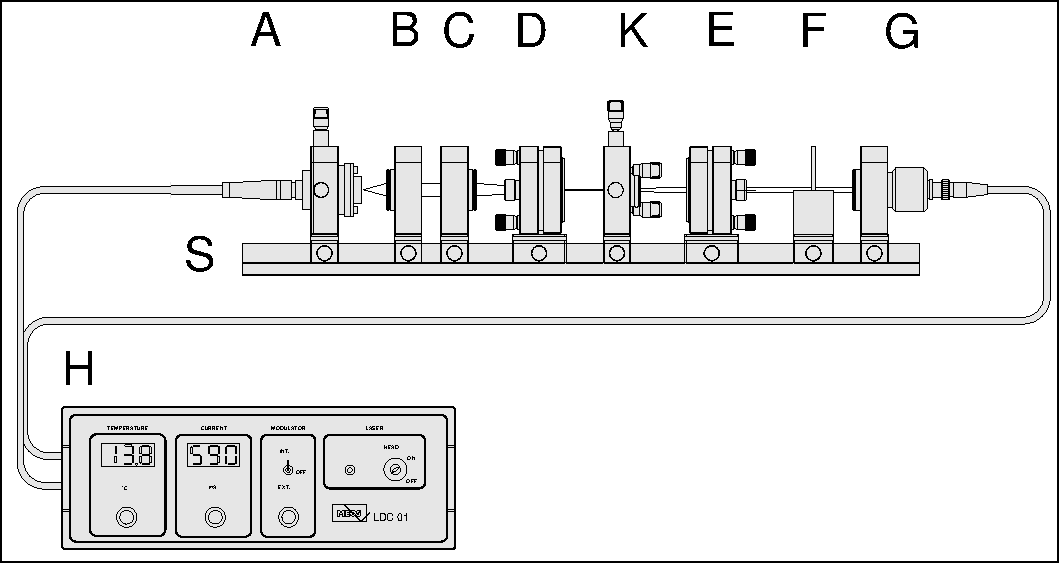
\includegraphics[width=0.9\textwidth]{setup_Nd_YAG_SHG.pdf}
	\caption[Setup for Second Harmonic Generation]{Setup for Second Harmonic Generation. A KTP crystal in a holder (K) for frequency doubling is set in midst of the Nd:YAG - resonator system. The filter (F) is replaced by a BG39 filter which absorbs infrared light and let the radiation at $\lambda=532\nano\metre$ pass. \cite{lit:manual}}
	\label{fig:setup_Nd:YAG_SHG}
\end{figure}

Since $P_\text{diode}$ is linear to the injection current $I$, and as proved in the previous section, $P_{1064}$ is linear to $P_\text{diode}$, we can plot the output power $P_{532}$ of the second harmonic generation against the fundamental power $P_{1064}$, as depicted in figure \ref{fig:P532}.

\begin{figure}[h]
	\centering
	% This file was created by matlab2tikz.
% Minimal pgfplots version: 1.3
%
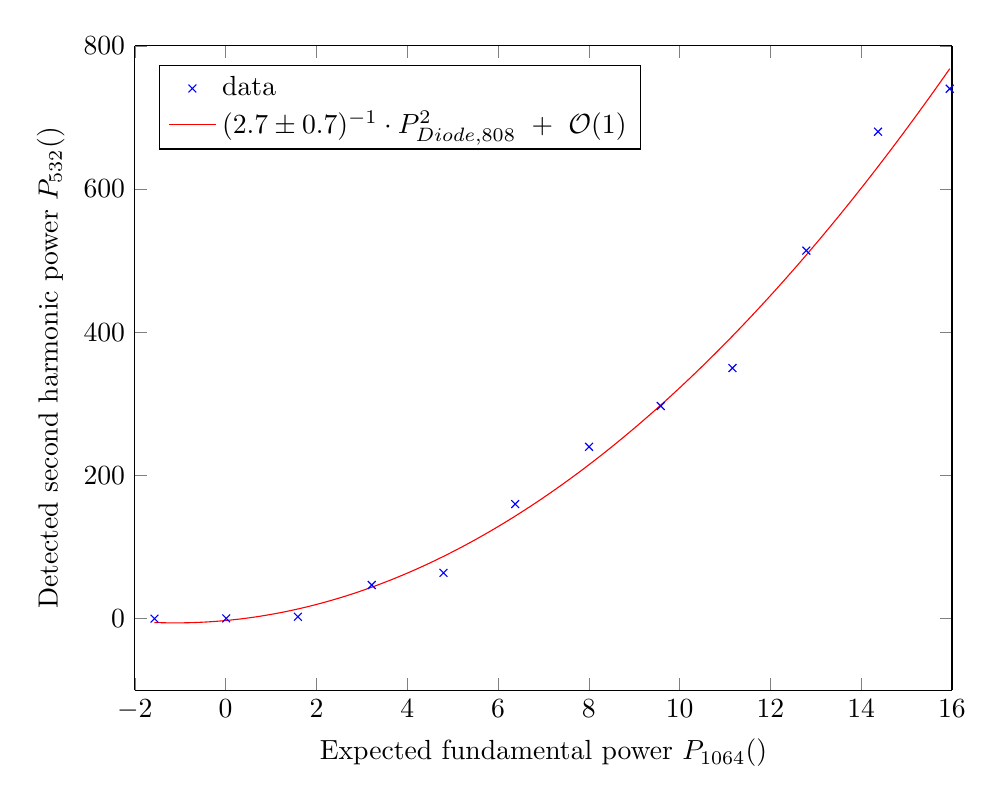
\begin{tikzpicture}

\begin{axis}[%
width=0.855828\textwidth,
height=0.675\textwidth,
at={(0\textwidth,0\textwidth)},
scale only axis,
separate axis lines,
every outer x axis line/.append style={black},
every x tick label/.append style={font=\color{black}},
xmin=-2,
xmax=16,
xlabel={Expected fundamental power $P_{1064}(\milli\watt)$},
every outer y axis line/.append style={black},
every y tick label/.append style={font=\color{black}},
ymin=-100,
ymax=800,
ylabel={Detected second harmonic power $P_{532}(\micro\watt)$},
legend style={at={(0.03,0.97)},anchor=north west,legend cell align=left,align=left,draw=black}
]
\addplot [color=blue,only marks,mark=x,mark options={solid}]
  table[row sep=crcr]{%
-1.56771622454173	0\\
0.0118188344330659	0.367\\
1.59135389340786	2.6\\
3.21875365113946	47\\
4.79828871011426	64\\
6.37782376908905	160\\
8.00522352682066	240\\
9.58475858579545	297\\
11.1642936447702	350\\
12.7916934025019	514\\
14.3712284614766	680\\
15.9507635204514	740\\
};
\addlegendentry{data};

\addplot [color=red,solid]
  table[row sep=crcr]{%
-1.56771622454173	-5.35281870966423\\
-1.55019774479674	-5.39450317918244\\
-1.53267926505174	-5.43455593530438\\
-1.51516078530675	-5.47297697803005\\
-1.49764230556176	-5.50976630735946\\
-1.48012382581676	-5.54492392329259\\
-1.46260534607177	-5.57844982582945\\
-1.44508686632678	-5.61034401497004\\
-1.42756838658178	-5.64060649071435\\
-1.41004990683679	-5.6692372530624\\
-1.3925314270918	-5.69623630201418\\
-1.3750129473468	-5.72160363756969\\
-1.35749446760181	-5.74533925972892\\
-1.33997598785682	-5.76744316849189\\
-1.32245750811182	-5.78791536385858\\
-1.30493902836683	-5.80675584582901\\
-1.28742054862184	-5.82396461440316\\
-1.26990206887684	-5.83954166958105\\
-1.25238358913185	-5.85348701136266\\
-1.23486510938686	-5.865800639748\\
-1.21734662964186	-5.87648255473707\\
-1.19982814989687	-5.88553275632987\\
-1.18230967015188	-5.8929512445264\\
-1.16479119040689	-5.89873801932666\\
-1.14727271066189	-5.90289308073065\\
-1.1297542309169	-5.90541642873837\\
-1.11223575117191	-5.90630806334982\\
-1.09471727142691	-5.905567984565\\
-1.07719879168192	-5.9031961923839\\
-1.05968031193693	-5.89919268680654\\
-1.04216183219193	-5.89355746783291\\
-1.02464335244694	-5.886290535463\\
-1.00712487270195	-5.87739188969683\\
-0.989606392956954	-5.86686153053438\\
-0.972087913211961	-5.85469945797566\\
-0.954569433466967	-5.84090567202068\\
-0.937050953721974	-5.82548017266942\\
-0.919532473976981	-5.80842295992189\\
-0.902013994231988	-5.78973403377809\\
-0.884495514486995	-5.76941339423802\\
-0.866977034742002	-5.74746104130168\\
-0.849458554997009	-5.72387697496907\\
-0.831940075252015	-5.69866119524019\\
-0.814421595507022	-5.67181370211504\\
-0.796903115762029	-5.64333449559362\\
-0.779384636017036	-5.61322357567592\\
-0.761866156272043	-5.58148094236196\\
-0.744347676527049	-5.54810659565172\\
-0.726829196782056	-5.51310053554522\\
-0.709310717037063	-5.47646276204244\\
-0.69179223729207	-5.4381932751434\\
-0.674273757547077	-5.39829207484808\\
-0.656755277802084	-5.35675916115649\\
-0.639236798057091	-5.31359453406864\\
-0.621718318312097	-5.26879819358451\\
-0.604199838567104	-5.22237013970411\\
-0.586681358822111	-5.17431037242744\\
-0.569162879077118	-5.1246188917545\\
-0.551644399332125	-5.07329569768529\\
-0.534125919587132	-5.02034079021981\\
-0.516607439842138	-4.96575416935805\\
-0.499088960097145	-4.90953583510003\\
-0.481570480352152	-4.85168578744574\\
-0.464052000607159	-4.79220402639518\\
-0.446533520862166	-4.73109055194834\\
-0.429015041117172	-4.66834536410524\\
-0.411496561372179	-4.60396846286586\\
-0.393978081627186	-4.53795984823021\\
-0.376459601882193	-4.4703195201983\\
-0.3589411221372	-4.40104747877011\\
-0.341422642392207	-4.33014372394565\\
-0.323904162647213	-4.25760825572492\\
-0.30638568290222	-4.18344107410793\\
-0.288867203157227	-4.10764217909465\\
-0.271348723412234	-4.03021157068511\\
-0.253830243667241	-3.9511492488793\\
-0.236311763922248	-3.87045521367722\\
-0.218793284177255	-3.78812946507887\\
-0.201274804432261	-3.70417200308425\\
-0.183756324687268	-3.61858282769335\\
-0.166237844942275	-3.53136193890619\\
-0.148719365197282	-3.44250933672276\\
-0.131200885452289	-3.35202502114305\\
-0.113682405707296	-3.25990899216708\\
-0.0961639259623024	-3.16616124979483\\
-0.0786454462173092	-3.07078179402631\\
-0.061126966472316	-2.97377062486153\\
-0.043608486727323	-2.87512774230047\\
-0.0260900069823298	-2.77485314634314\\
-0.00857152723733656	-2.67294683698954\\
0.00894695250765665	-2.56940881423967\\
0.0118188344330659	-2.55227969514988\\
0.0264654322526499	-2.46423907809353\\
0.0439839119976428	-2.35743762855112\\
0.0615023917426361	-2.24900446561244\\
0.0790208714876293	-2.13893958927749\\
0.0965393512326225	-2.02724299954626\\
0.114057830977615	-1.91391469641877\\
0.131576310722609	-1.79895467989501\\
0.149094790467602	-1.68236294997497\\
0.166613270212595	-1.56413950665867\\
0.184131749957588	-1.44428434994609\\
0.201650229702581	-1.32279747983725\\
0.219168709447574	-1.19967889633213\\
0.236687189192568	-1.07492859943074\\
0.254205668937561	-0.948546589133082\\
0.271724148682554	-0.820532865439154\\
0.289242628427547	-0.690887428348956\\
0.30676110817254	-0.559610277862486\\
0.324279587917534	-0.426701413979745\\
0.341798067662527	-0.292160836700734\\
0.35931654740752	-0.155988546025452\\
0.376835027152513	-0.0181845419539011\\
0.394353506897506	0.121251175513922\\
0.411871986642499	0.262318606378015\\
0.429390466387493	0.40501775063838\\
0.446908946132486	0.549348608295015\\
0.464427425877479	0.695311179347918\\
0.481945905622472	0.842905463797096\\
0.499464385367465	0.992131461642541\\
0.516982865112458	1.14298917288426\\
0.534501344857452	1.29547859752225\\
0.552019824602445	1.4495997355565\\
0.569538304347438	1.60535258698703\\
0.587056784092431	1.76273715181383\\
0.604575263837424	1.9217534300369\\
0.622093743582417	2.08240142165624\\
0.63961222332741	2.24468112667185\\
0.657130703072404	2.40859254508374\\
0.674649182817397	2.57413567689189\\
0.69216766256239	2.74131052209631\\
0.709686142307383	2.910117080697\\
0.727204622052376	3.08055535269397\\
0.74472310179737	3.2526253380872\\
0.762241581542363	3.42632703687671\\
0.779760061287356	3.60166044906248\\
0.797278541032349	3.77862557464453\\
0.814797020777342	3.95722241362284\\
0.832315500522335	4.13745096599743\\
0.849833980267328	4.31931123176829\\
0.867352460012321	4.50280321093542\\
0.884870939757315	4.68792690349882\\
0.902389419502308	4.87468230945849\\
0.919907899247301	5.06306942881443\\
0.937426378992294	5.25308826156664\\
0.954944858737287	5.44473880771512\\
0.972463338482281	5.63802106725988\\
0.989981818227274	5.83293504020089\\
1.00750029797227	6.02948072653819\\
1.02501877771726	6.22765812627175\\
1.04253725746225	6.42746723940159\\
1.06005573720725	6.62890806592769\\
1.07757421695224	6.83198060585007\\
1.09509269669723	7.03668485916872\\
1.11261117644223	7.24302082588363\\
1.13012965618722	7.45098850599482\\
1.14764813593221	7.66058789950228\\
1.16516661567721	7.87181900640601\\
1.1826850954222	8.08468182670601\\
1.20020357516719	8.29917636040228\\
1.21772205491218	8.51530260749481\\
1.23524053465718	8.73306056798363\\
1.25275901440217	8.95245024186871\\
1.27027749414716	9.17347162915006\\
1.28779597389216	9.39612472982768\\
1.30531445363715	9.62040954390158\\
1.32283293338214	9.84632607137174\\
1.34035141312714	10.0738743122382\\
1.35786989287213	10.3030542665009\\
1.37538837261712	10.5338659341599\\
1.39290685236212	10.7663093152151\\
1.41042533210711	11.0003844096666\\
1.4279438118521	11.2360912175144\\
1.4454622915971	11.4734297387585\\
1.46298077134209	11.7123999733988\\
1.48049925108708	11.9530019214354\\
1.49801773083208	12.1952355828683\\
1.51553621057707	12.4391009576974\\
1.53305469032206	12.6845980459228\\
1.55057317006706	12.9317268475445\\
1.56809164981205	13.1804873625624\\
1.58561012955704	13.4308795909767\\
1.59135389340786	13.5133306005215\\
1.60312860930203	13.6829035327872\\
1.62064708904703	13.9365591879939\\
1.63816556879202	14.191846556597\\
1.65568404853701	14.4487656385963\\
1.67320252828201	14.7073164339918\\
1.690721008027	14.9674989427837\\
1.70823948777199	15.2293131649718\\
1.72575796751699	15.4927591005562\\
1.74327644726198	15.7578367495369\\
1.76079492700697	16.0245461119138\\
1.77831340675197	16.292887187687\\
1.79583188649696	16.5628599768565\\
1.81335036624195	16.8344644794222\\
1.83086884598695	17.1077006953842\\
1.84838732573194	17.3825686247425\\
1.86590580547693	17.659068267497\\
1.88342428522193	17.9371996236479\\
1.90094276496692	18.216962693195\\
1.91846124471191	18.4983574761383\\
1.9359797244569	18.781383972478\\
1.9534982042019	19.0660421822139\\
1.97101668394689	19.352332105346\\
1.98853516369188	19.6402537418745\\
2.00605364343688	19.9298070917992\\
2.02357212318187	20.2209921551202\\
2.04109060292686	20.5138089318374\\
2.05860908267186	20.808257421951\\
2.07612756241685	21.1043376254608\\
2.09364604216184	21.4020495423668\\
2.11116452190684	21.7013931726692\\
2.12868300165183	22.0023685163678\\
2.14620148139682	22.3049755734627\\
2.16371996114182	22.6092143439538\\
2.18123844088681	22.9150848278412\\
2.1987569206318	23.2225870251249\\
2.2162754003768	23.5317209358049\\
2.23379388012179	23.8424865598811\\
2.25131235986678	24.1548838973537\\
2.26883083961177	24.4689129482224\\
2.28634931935677	24.7845737124875\\
2.30386779910176	25.1018661901488\\
2.32138627884675	25.4207903812064\\
2.33890475859175	25.7413462856602\\
2.35642323833674	26.0635339035104\\
2.37394171808173	26.3873532347568\\
2.39146019782673	26.7128042793994\\
2.40897867757172	27.0398870374384\\
2.42649715731671	27.3686015088736\\
2.44401563706171	27.6989476937051\\
2.4615341168067	28.0309255919328\\
2.47905259655169	28.3645352035568\\
2.49657107629669	28.6997765285771\\
2.51408955604168	29.0366495669937\\
2.53160803578667	29.3751543188065\\
2.54912651553167	29.7152907840156\\
2.56664499527666	30.057058962621\\
2.58416347502165	30.4004588546227\\
2.60168195476664	30.7454904600206\\
2.61920043451164	31.0921537788148\\
2.63671891425663	31.4404488110052\\
2.65423739400162	31.790375556592\\
2.67175587374662	32.141934015575\\
2.68927435349161	32.4951241879542\\
2.7067928332366	32.8499460737298\\
2.7243113129816	33.2063996729016\\
2.74182979272659	33.5644849854697\\
2.75934827247158	33.924202011434\\
2.77686675221658	34.2855507507946\\
2.79438523196157	34.6485312035515\\
2.81190371170656	35.0131433697047\\
2.82942219145156	35.3793872492541\\
2.84694067119655	35.7472628421998\\
2.86445915094154	36.1167701485418\\
2.88197763068654	36.4879091682801\\
2.89949611043153	36.8606799014146\\
2.91701459017652	37.2350823479454\\
2.93453306992151	37.6111165078724\\
2.95205154966651	37.9887823811957\\
2.9695700294115	38.3680799679154\\
2.98708850915649	38.7490092680312\\
3.00460698890149	39.1315702815434\\
3.02212546864648	39.5157630084518\\
3.03964394839147	39.9015874487564\\
3.05716242813647	40.2890436024574\\
3.07468090788146	40.6781314695546\\
3.09219938762645	41.0688510500481\\
3.10971786737145	41.4612023439379\\
3.12723634711644	41.8551853512239\\
3.14475482686143	42.2508000719062\\
3.16227330660643	42.6480465059848\\
3.17979178635142	43.0469246534596\\
3.19731026609641	43.4474345143308\\
3.21482874584141	43.8495760885981\\
3.21875365113946	43.9398971211654\\
3.2323472255864	44.2533493762618\\
3.24986570533139	44.6587543773217\\
3.26738418507639	45.0657910917779\\
3.28490266482138	45.4744595196304\\
3.30242114456637	45.8847596608791\\
3.31993962431137	46.2966915155242\\
3.33745810405636	46.7102550835655\\
3.35497658380135	47.125450365003\\
3.37249506354634	47.5422773598368\\
3.39001354329134	47.9607360680669\\
3.40753202303633	48.3808264896933\\
3.42505050278132	48.8025486247159\\
3.44256898252632	49.2259024731348\\
3.46008746227131	49.65088803495\\
3.4776059420163	50.0775053101614\\
3.4951244217613	50.5057542987692\\
3.51264290150629	50.9356350007732\\
3.53016138125128	51.3671474161734\\
3.54767986099628	51.8002915449699\\
3.56519834074127	52.2350673871627\\
3.58271682048626	52.6714749427518\\
3.60023530023126	53.1095142117371\\
3.61775377997625	53.5491851941188\\
3.63527225972124	53.9904878898966\\
3.65279073946623	54.4334222990708\\
3.67030921921123	54.8779884216412\\
3.68782769895622	55.3241862576079\\
3.70534617870121	55.7720158069709\\
3.72286465844621	56.2214770697301\\
3.7403831381912	56.6725700458856\\
3.75790161793619	57.1252947354374\\
3.77542009768119	57.5796511383854\\
3.79293857742618	58.0356392547298\\
3.81045705717117	58.4932590844703\\
3.82797553691617	58.9525106276072\\
3.84549401666116	59.4133938841403\\
3.86301249640615	59.8759088540697\\
3.88053097615115	60.3400555373954\\
3.89804945589614	60.8058339341173\\
3.91556793564113	61.2732440442356\\
3.93308641538613	61.74228586775\\
3.95060489513112	62.2129594046608\\
3.96812337487611	62.6852646549678\\
3.9856418546211	63.1592016186711\\
4.0031603343661	63.6347702957707\\
4.02067881411109	64.1119706862665\\
4.03819729385608	64.5908027901586\\
4.05571577360108	65.071266607447\\
4.07323425334607	65.5533621381316\\
4.09075273309106	66.0370893822125\\
4.10827121283606	66.5224483396897\\
4.12578969258105	67.0094390105632\\
4.14330817232604	67.4980613948329\\
4.16082665207104	67.9883154924989\\
4.17834513181603	68.4802013035612\\
4.19586361156102	68.9737188280198\\
4.21338209130602	69.4688680658745\\
4.23090057105101	69.9656490171256\\
4.248419050796	70.464061681773\\
4.265937530541	70.9641060598166\\
4.28345601028599	71.4657821512565\\
4.30097449003098	71.9690899560927\\
4.31849296977598	72.4740294743251\\
4.33601144952097	72.9806007059538\\
4.35352992926596	73.4888036509788\\
4.37104840901095	73.9986383094\\
4.38856688875595	74.5101046812176\\
4.40608536850094	75.0232027664313\\
4.42360384824593	75.5379325650414\\
4.44112232799093	76.0542940770477\\
4.45864080773592	76.5722873024503\\
4.47615928748091	77.0919122412492\\
4.49367776722591	77.6131688934443\\
4.5111962469709	78.1360572590357\\
4.52871472671589	78.6605773380234\\
4.54623320646089	79.1867291304074\\
4.56375168620588	79.7145126361876\\
4.58127016595087	80.2439278553641\\
4.59878864569587	80.7749747879369\\
4.61630712544086	81.3076534339059\\
4.63382560518585	81.8419637932712\\
4.65134408493085	82.3779058660328\\
4.66886256467584	82.9154796521906\\
4.68638104442083	83.4546851517447\\
4.70389952416582	83.9955223646951\\
4.72141800391082	84.5379912910418\\
4.73893648365581	85.0820919307847\\
4.7564549634008	85.6278242839239\\
4.7739734431458	86.1751883504594\\
4.79149192289079	86.7241841303911\\
4.79828871011426	86.9376218361556\\
4.80901040263578	87.2748116237191\\
4.82652888238078	87.8270708304434\\
4.84404736212577	88.380961750564\\
4.86156584187076	88.9364843840808\\
4.87908432161576	89.4936387309939\\
4.89660280136075	90.0524247913033\\
4.91412128110574	90.6128425650089\\
4.93163976085074	91.1748920521108\\
4.94915824059573	91.738573252609\\
4.96667672034072	92.3038861665034\\
4.98419520008572	92.8708307937942\\
5.00171367983071	93.4394071344811\\
5.0192321595757	94.0096151885644\\
5.03675063932069	94.5814549560439\\
5.05426911906569	95.1549264369197\\
5.07178759881068	95.7300296311918\\
5.08930607855567	96.3067645388601\\
5.10682455830067	96.8851311599247\\
5.12434303804566	97.4651294943856\\
5.14186151779065	98.0467595422428\\
5.15937999753565	98.6300213034962\\
5.17689847728064	99.2149147781459\\
5.19441695702563	99.8014399661919\\
5.21193543677063	100.389596867634\\
5.22945391651562	100.979385482473\\
5.24697239626061	101.570805810707\\
5.26449087600561	102.163857852338\\
5.2820093557506	102.758541607366\\
5.29952783549559	103.354857075789\\
5.31704631524059	103.952804257609\\
5.33456479498558	104.552383152825\\
5.35208327473057	105.153593761438\\
5.36960175447557	105.756436083446\\
5.38712023422056	106.360910118851\\
5.40463871396555	106.967015867653\\
5.42215719371054	107.57475332985\\
5.43967567345554	108.184122505444\\
5.45719415320053	108.795123394434\\
5.47471263294552	109.40775599682\\
5.49223111269052	110.022020312603\\
5.50974959243551	110.637916341781\\
5.5272680721805	111.255444084357\\
5.5447865519255	111.874603540328\\
5.56230503167049	112.495394709696\\
5.57982351141548	113.11781759246\\
5.59734199116048	113.74187218862\\
5.61486047090547	114.367558498176\\
5.63237895065046	114.994876521129\\
5.64989743039546	115.623826257478\\
5.66741591014045	116.254407707223\\
5.68493438988544	116.886620870365\\
5.70245286963044	117.520465746903\\
5.71997134937543	118.155942336837\\
5.73748982912042	118.793050640167\\
5.75500830886541	119.431790656894\\
5.77252678861041	120.072162387016\\
5.7900452683554	120.714165830536\\
5.80756374810039	121.357800987451\\
5.82508222784539	122.003067857763\\
5.84260070759038	122.649966441471\\
5.86011918733537	123.298496738575\\
5.87763766708037	123.948658749076\\
5.89515614682536	124.600452472972\\
5.91267462657035	125.253877910265\\
5.93019310631535	125.908935060955\\
5.94771158606034	126.56562392504\\
5.96523006580533	127.223944502522\\
5.98274854555033	127.8838967934\\
6.00026702529532	128.545480797675\\
6.01778550504031	129.208696515345\\
6.0353039847853	129.873543946412\\
6.0528224645303	130.540023090876\\
6.07034094427529	131.208133948735\\
6.08785942402028	131.877876519991\\
6.10537790376528	132.549250804643\\
6.12289638351027	133.222256802691\\
6.14041486325526	133.896894514136\\
6.15793334300026	134.573163938977\\
6.17545182274525	135.251065077214\\
6.19297030249024	135.930597928847\\
6.21048878223524	136.611762493877\\
6.22800726198023	137.294558772303\\
6.24552574172522	137.978986764125\\
6.26304422147022	138.665046469343\\
6.28056270121521	139.352737887958\\
6.2980811809602	140.042061019969\\
6.3155996607052	140.733015865376\\
6.33311814045019	141.42560242418\\
6.35063662019518	142.11982069638\\
6.36815509994018	142.815670681976\\
6.37782376908905	143.200417832303\\
6.38567357968517	143.513152380968\\
6.40319205943016	144.212265793357\\
6.42071053917515	144.913010919142\\
6.43822901892015	145.615387758323\\
6.45574749866514	146.3193963109\\
6.47326597841013	147.025036576874\\
6.49078445815513	147.732308556244\\
6.50830293790012	148.44121224901\\
6.52582141764511	149.151747655173\\
6.54333989739011	149.863914774732\\
6.5608583771351	150.577713607687\\
6.57837685688009	151.293144154038\\
6.59589533662509	152.010206413786\\
6.61341381637008	152.72890038693\\
6.63093229611507	153.44922607347\\
6.64845077586007	154.171183473406\\
6.66596925560506	154.894772586739\\
6.68348773535005	155.619993413468\\
6.70100621509505	156.346845953593\\
6.71852469484004	157.075330207115\\
6.73604317458503	157.805446174032\\
6.75356165433002	158.537193854346\\
6.77108013407502	159.270573248057\\
6.78859861382001	160.005584355163\\
6.80611709356501	160.742227175666\\
6.82363557331	161.480501709565\\
6.84115405305499	162.220407956861\\
6.85867253279998	162.961945917552\\
6.87619101254498	163.70511559164\\
6.89370949228997	164.449916979125\\
6.91122797203496	165.196350080005\\
6.92874645177996	165.944414894282\\
6.94626493152495	166.694111421955\\
6.96378341126994	167.445439663024\\
6.98130189101494	168.19839961749\\
6.99882037075993	168.952991285352\\
7.01633885050492	169.70921466661\\
7.03385733024992	170.467069761264\\
7.05137580999491	171.226556569315\\
7.0688942897399	171.987675090762\\
7.08641276948489	172.750425325605\\
7.10393124922989	173.514807273844\\
7.12144972897488	174.28082093548\\
7.13896820871988	175.048466310512\\
7.15648668846487	175.81774339894\\
7.17400516820986	176.588652200765\\
7.19152364795485	177.361192715986\\
7.20904212769985	178.135364944603\\
7.22656060744484	178.911168886616\\
7.24407908718983	179.688604542026\\
7.26159756693483	180.467671910831\\
7.27911604667982	181.248370993034\\
7.29663452642481	182.030701788632\\
7.31415300616981	182.814664297627\\
7.3316714859148	183.600258520018\\
7.34918996565979	184.387484455805\\
7.36670844540479	185.176342104989\\
7.38422692514978	185.966831467568\\
7.40174540489477	186.758952543544\\
7.41926388463976	187.552705332917\\
7.43678236438476	188.348089835685\\
7.45430084412975	189.14510605185\\
7.47181932387474	189.943753981411\\
7.48933780361974	190.744033624369\\
7.50685628336473	191.545944980722\\
7.52437476310972	192.349488050472\\
7.54189324285472	193.154662833619\\
7.55941172259971	193.961469330161\\
7.5769302023447	194.7699075401\\
7.5944486820897	195.579977463435\\
7.61196716183469	196.391679100166\\
7.62948564157968	197.205012450294\\
7.64700412132468	198.019977513818\\
7.66452260106967	198.836574290738\\
7.68204108081466	199.654802781054\\
7.69955956055966	200.474662984767\\
7.71707804030465	201.296154901876\\
7.73459652004964	202.119278532381\\
7.75211499979464	202.944033876282\\
7.76963347953963	203.77042093358\\
7.78715195928462	204.598439704274\\
7.80467043902961	205.428090188364\\
7.82218891877461	206.259372385851\\
7.8397073985196	207.092286296734\\
7.8572258782646	207.926831921013\\
7.87474435800959	208.763009258688\\
7.89226283775458	209.60081830976\\
7.90978131749957	210.440259074228\\
7.92729979724457	211.281331552092\\
7.94481827698956	212.124035743352\\
7.96233675673455	212.968371648009\\
7.97985523647955	213.814339266062\\
7.99737371622454	214.661938597511\\
8.00522352682066	215.042266589801\\
8.01489219596953	215.511169642357\\
8.03241067571453	216.362032400599\\
8.04992915545952	217.214526872237\\
8.06744763520451	218.068653057271\\
8.08496611494951	218.924410955702\\
8.1024845946945	219.781800567529\\
8.12000307443949	220.640821892752\\
8.13752155418448	221.501474931371\\
8.15504003392948	222.363759683387\\
8.17255851367447	223.227676148799\\
8.19007699341946	224.093224327607\\
8.20759547316446	224.960404219812\\
8.22511395290945	225.829215825412\\
8.24263243265444	226.699659144409\\
8.26015091239944	227.571734176803\\
8.27766939214443	228.445440922592\\
8.29518787188942	229.320779381778\\
8.31270635163442	230.19774955436\\
8.33022483137941	231.076351440339\\
8.3477433111244	231.956585039713\\
8.3652617908694	232.838450352484\\
8.38278027061439	233.721947378652\\
8.40029875035938	234.607076118215\\
8.41781723010438	235.493836571175\\
8.43533570984937	236.382228737531\\
8.45285418959436	237.272252617283\\
8.47037266933935	238.163908210432\\
8.48789114908435	239.057195516977\\
8.50540962882934	239.952114536918\\
8.52292810857433	240.848665270255\\
8.54044658831933	241.746847716989\\
8.55796506806432	242.646661877119\\
8.57548354780931	243.548107750645\\
8.59300202755431	244.451185337567\\
8.6105205072993	245.355894637886\\
8.62803898704429	246.262235651601\\
8.64555746678929	247.170208378712\\
8.66307594653428	248.07981281922\\
8.68059442627927	248.991048973124\\
8.69811290602427	249.903916840424\\
8.71563138576926	250.81841642112\\
8.73314986551425	251.734547715213\\
8.75066834525925	252.652310722702\\
8.76818682500424	253.571705443587\\
8.78570530474923	254.492731877868\\
8.80322378449423	255.415390025546\\
8.82074226423922	256.33967988662\\
8.83826074398421	257.26560146109\\
8.8557792237292	258.193154748956\\
8.8732977034742	259.122339750219\\
8.89081618321919	260.053156464878\\
8.90833466296418	260.985604892934\\
8.92585314270918	261.919685034385\\
8.94337162245417	262.855396889233\\
8.96089010219916	263.792740457477\\
8.97840858194416	264.731715739118\\
8.99592706168915	265.672322734154\\
9.01344554143414	266.614561442587\\
9.03096402117914	267.558431864417\\
9.04848250092413	268.503933999642\\
9.06600098066912	269.451067848264\\
9.08351946041412	270.399833410282\\
9.10103794015911	271.350230685696\\
9.1185564199041	272.302259674507\\
9.1360748996491	273.255920376714\\
9.15359337939409	274.211212792317\\
9.17111185913908	275.168136921316\\
9.18863033888407	276.126692763712\\
9.20614881862907	277.086880319504\\
9.22366729837406	278.048699588692\\
9.24118577811905	279.012150571276\\
9.25870425786405	279.977233267257\\
9.27622273760904	280.943947676634\\
9.29374121735403	281.912293799407\\
9.31125969709903	282.882271635577\\
9.32877817684402	283.853881185143\\
9.34629665658901	284.827122448105\\
9.36381513633401	285.801995424463\\
9.381333616079	286.778500114218\\
9.39885209582399	287.756636517369\\
9.41637057556899	288.736404633916\\
9.43388905531398	289.717804463859\\
9.45140753505897	290.700836007199\\
9.46892601480397	291.685499263935\\
9.48644449454896	292.671794234067\\
9.50396297429395	293.659720917596\\
9.52148145403894	294.649279314521\\
9.53899993378394	295.640469424842\\
9.55651841352893	296.633291248559\\
9.57403689327392	297.627744785673\\
9.58475858579545	298.237177005267\\
9.59155537301892	298.623830036183\\
9.60907385276391	299.621547000089\\
9.6265923325089	300.620895677391\\
9.6441108122539	301.62187606809\\
9.66162929199889	302.624488172185\\
9.67914777174388	303.628731989676\\
9.69666625148888	304.634607520564\\
9.71418473123387	305.642114764847\\
9.73170321097886	306.651253722527\\
9.74922169072386	307.662024393604\\
9.76674017046885	308.674426778076\\
9.78425865021384	309.688460875945\\
9.80177712995884	310.70412668721\\
9.81929560970383	311.721424211872\\
9.83681408944882	312.740353449929\\
9.85433256919382	313.760914401383\\
9.87185104893881	314.783107066234\\
9.8893695286838	315.80693144448\\
9.90688800842879	316.832387536123\\
9.92440648817379	317.859475341162\\
9.94192496791878	318.888194859597\\
9.95944344766377	319.918546091429\\
9.97696192740877	320.950529036657\\
9.99448040715376	321.984143695281\\
10.0119988868988	323.019390067301\\
10.0295173666437	324.056268152718\\
10.0470358463887	325.094777951531\\
10.0645543261337	326.13491946374\\
10.0820728058787	327.176692689345\\
10.0995912856237	328.220097628347\\
10.1171097653687	329.265134280745\\
10.1346282451137	330.311802646539\\
10.1521467248587	331.36010272573\\
10.1696652046037	332.410034518317\\
10.1871836843487	333.4615980243\\
10.2047021640937	334.514793243679\\
10.2222206438387	335.569620176455\\
10.2397391235837	336.626078822627\\
10.2572576033287	337.684169182195\\
10.2747760830737	338.743891255159\\
10.2922945628186	339.80524504152\\
10.3098130425636	340.868230541277\\
10.3273315223086	341.93284775443\\
10.3448500020536	342.99909668098\\
10.3623684817986	344.066977320925\\
10.3798869615436	345.136489674267\\
10.3974054412886	346.207633741006\\
10.4149239210336	347.28040952114\\
10.4324424007786	348.354817014671\\
10.4499608805236	349.430856221598\\
10.4674793602686	350.508527141922\\
10.4849978400136	351.587829775642\\
10.5025163197586	352.668764122757\\
10.5200347995036	353.75133018327\\
10.5375532792485	354.835527957178\\
10.5550717589935	355.921357444483\\
10.5725902387385	357.008818645184\\
10.5901087184835	358.097911559281\\
10.6076271982285	359.188636186775\\
10.6251456779735	360.280992527665\\
10.6426641577185	361.374980581951\\
10.6601826374635	362.470600349633\\
10.6777011172085	363.567851830712\\
10.6952195969535	364.666735025187\\
10.7127380766985	365.767249933058\\
10.7302565564435	366.869396554325\\
10.7477750361885	367.973174888989\\
10.7652935159335	369.078584937049\\
10.7828119956785	370.185626698505\\
10.8003304754234	371.294300173358\\
10.8178489551684	372.404605361607\\
10.8353674349134	373.516542263252\\
10.8528859146584	374.630110878293\\
10.8704043944034	375.745311206731\\
10.8879228741484	376.862143248565\\
10.9054413538934	377.980607003795\\
10.9229598336384	379.100702472422\\
10.9404783133834	380.222429654444\\
10.9579967931284	381.345788549863\\
10.9755152728734	382.470779158678\\
10.9930337526184	383.59740148089\\
11.0105522323634	384.725655516498\\
11.0280707121084	385.855541265502\\
11.0455891918534	386.987058727902\\
11.0631076715983	388.120207903699\\
11.0806261513433	389.254988792892\\
11.0981446310883	390.391401395481\\
11.1156631108333	391.529445711466\\
11.1331815905783	392.669121740848\\
11.1507000703233	393.810429483626\\
11.1642936447702	394.69715870189\\
11.1682185500683	394.9533689398\\
11.1857370298133	396.097940109371\\
11.2032555095583	397.244142992338\\
11.2207739893033	398.391977588701\\
11.2382924690483	399.54144389846\\
11.2558109487933	400.692541921615\\
11.2733294285383	401.845271658167\\
11.2908479082833	402.999633108115\\
11.3083663880282	404.15562627146\\
11.3258848677732	405.3132511482\\
11.3434033475182	406.472507738337\\
11.3609218272632	407.633396041871\\
11.3784403070082	408.7959160588\\
11.3959587867532	409.960067789126\\
11.4134772664982	411.125851232848\\
11.4309957462432	412.293266389966\\
11.4485142259882	413.462313260481\\
11.4660327057332	414.632991844392\\
11.4835511854782	415.805302141699\\
11.5010696652232	416.979244152402\\
11.5185881449682	418.154817876502\\
11.5361066247132	419.332023313998\\
11.5536251044582	420.51086046489\\
11.5711435842031	421.691329329178\\
11.5886620639481	422.873429906863\\
11.6061805436931	424.057162197944\\
11.6236990234381	425.242526202421\\
11.6412175031831	426.429521920295\\
11.6587359829281	427.618149351565\\
11.6762544626731	428.808408496231\\
11.6937729424181	430.000299354293\\
11.7112914221631	431.193821925752\\
11.7288099019081	432.388976210607\\
11.7463283816531	433.585762208858\\
11.7638468613981	434.784179920505\\
11.7813653411431	435.984229345549\\
11.7988838208881	437.185910483989\\
11.816402300633	438.389223335825\\
11.833920780378	439.594167901058\\
11.851439260123	440.800744179686\\
11.868957739868	442.008952171711\\
11.886476219613	443.218791877133\\
11.903994699358	444.43026329595\\
11.921513179103	445.643366428164\\
11.939031658848	446.858101273775\\
11.956550138593	448.074467832781\\
11.974068618338	449.292466105184\\
11.991587098083	450.512096090982\\
12.009105577828	451.733357790178\\
12.026624057573	452.956251202769\\
12.044142537318	454.180776328757\\
12.061661017063	455.406933168141\\
12.0791794968079	456.634721720921\\
12.0966979765529	457.864141987098\\
12.1142164562979	459.095193966671\\
12.1317349360429	460.32787765964\\
12.1492534157879	461.562193066005\\
12.1667718955329	462.798140185767\\
12.1842903752779	464.035719018925\\
12.2018088550229	465.274929565479\\
12.2193273347679	466.515771825429\\
12.2368458145129	467.758245798776\\
12.2543642942579	469.002351485519\\
12.2718827740029	470.248088885659\\
12.2894012537479	471.495457999194\\
12.3069197334929	472.744458826126\\
12.3244382132379	473.995091366454\\
12.3419566929828	475.247355620178\\
12.3594751727278	476.501251587299\\
12.3769936524728	477.756779267816\\
12.3945121322178	479.013938661729\\
12.4120306119628	480.272729769039\\
12.4295490917078	481.533152589744\\
12.4470675714528	482.795207123846\\
12.4645860511978	484.058893371345\\
12.4821045309428	485.324211332239\\
12.4996230106878	486.59116100653\\
12.5171414904328	487.859742394217\\
12.5346599701778	489.1299554953\\
12.5521784499228	490.40180030978\\
12.5696969296678	491.675276837656\\
12.5872154094127	492.950385078928\\
12.6047338891577	494.227125033596\\
12.6222523689027	495.505496701661\\
12.6397708486477	496.785500083122\\
12.6572893283927	498.067135177979\\
12.6748078081377	499.350401986233\\
12.6923262878827	500.635300507883\\
12.7098447676277	501.921830742929\\
12.7273632473727	503.209992691371\\
12.7448817271177	504.49978635321\\
12.7624002068627	505.791211728444\\
12.7799186866077	507.084268817076\\
12.7916934025019	507.954289696242\\
12.7974371663527	508.378957619103\\
12.8149556460977	509.675278134527\\
12.8324741258427	510.973230363347\\
12.8499926055876	512.272814305563\\
12.8675110853326	513.574029961175\\
12.8850295650776	514.876877330184\\
12.9025480448226	516.181356412589\\
12.9200665245676	517.48746720839\\
12.9375850043126	518.795209717588\\
12.9551034840576	520.104583940182\\
12.9726219638026	521.415589876172\\
12.9901404435476	522.728227525558\\
13.0076589232926	524.042496888341\\
13.0251774030376	525.35839796452\\
13.0426958827826	526.675930754095\\
13.0602143625276	527.995095257066\\
13.0777328422726	529.315891473434\\
13.0952513220176	530.638319403198\\
13.1127698017625	531.962379046358\\
13.1302882815075	533.288070402915\\
13.1478067612525	534.615393472868\\
13.1653252409975	535.944348256217\\
13.1828437207425	537.274934752962\\
13.2003622004875	538.607152963104\\
13.2178806802325	539.941002886642\\
13.2353991599775	541.276484523576\\
13.2529176397225	542.613597873906\\
13.2704361194675	543.952342937633\\
13.2879545992125	545.292719714756\\
13.3054730789575	546.634728205275\\
13.3229915587025	547.978368409191\\
13.3405100384475	549.323640326503\\
13.3580285181924	550.670543957211\\
13.3755469979374	552.019079301315\\
13.3930654776824	553.369246358816\\
13.4105839574274	554.721045129712\\
13.4281024371724	556.074475614006\\
13.4456209169174	557.429537811695\\
13.4631393966624	558.786231722781\\
13.4806578764074	560.144557347263\\
13.4981763561524	561.504514685141\\
13.5156948358974	562.866103736415\\
13.5332133156424	564.229324501086\\
13.5507317953874	565.594176979153\\
13.5682502751324	566.960661170617\\
13.5857687548774	568.328777075476\\
13.6032872346224	569.698524693732\\
13.6208057143673	571.069904025384\\
13.6383241941123	572.442915070432\\
13.6558426738573	573.817557828877\\
13.6733611536023	575.193832300718\\
13.6908796333473	576.571738485955\\
13.7083981130923	577.951276384589\\
13.7259165928373	579.332445996618\\
13.7434350725823	580.715247322044\\
13.7609535523273	582.099680360867\\
13.7784720320723	583.485745113085\\
13.7959905118173	584.8734415787\\
13.8135089915623	586.262769757711\\
13.8310274713073	587.653729650119\\
13.8485459510523	589.046321255922\\
13.8660644307973	590.440544575122\\
13.8835829105422	591.836399607718\\
13.9011013902872	593.233886353711\\
13.9186198700322	594.6330048131\\
13.9361383497772	596.033754985884\\
13.9536568295222	597.436136872066\\
13.9711753092672	598.840150471643\\
13.9886937890122	600.245795784617\\
14.0062122687572	601.653072810987\\
14.0237307485022	603.061981550753\\
14.0412492282472	604.472522003916\\
14.0587677079922	605.884694170475\\
14.0762861877372	607.29849805043\\
14.0938046674822	608.713933643782\\
14.1113231472272	610.131000950529\\
14.1288416269721	611.549699970673\\
14.1463601067171	612.970030704213\\
14.1638785864621	614.39199315115\\
14.1813970662071	615.815587311483\\
14.1989155459521	617.240813185212\\
14.2164340256971	618.667670772337\\
14.2339525054421	620.096160072859\\
14.2514709851871	621.526281086777\\
14.2689894649321	622.958033814091\\
14.2865079446771	624.391418254801\\
14.3040264244221	625.826434408908\\
14.3215449041671	627.263082276411\\
14.3390633839121	628.70136185731\\
14.3565818636571	630.141273151605\\
14.3712284614766	631.346385812184\\
14.3741003434021	631.582816159297\\
14.391618823147	633.025990880385\\
14.409137302892	634.470797314869\\
14.426655782637	635.91723546275\\
14.444174262382	637.365305324027\\
14.461692742127	638.8150068987\\
14.479211221872	640.26634018677\\
14.496729701617	641.719305188235\\
14.514248181362	643.173901903097\\
14.531766661107	644.630130331355\\
14.549285140852	646.08799047301\\
14.566803620597	647.54748232806\\
14.584322100342	649.008605896507\\
14.601840580087	650.471361178351\\
14.619359059832	651.93574817359\\
14.6368775395769	653.401766882226\\
14.6543960193219	654.869417304258\\
14.6719144990669	656.338699439686\\
14.6894329788119	657.809613288511\\
14.7069514585569	659.282158850732\\
14.7244699383019	660.756336126349\\
14.7419884180469	662.232145115362\\
14.7595068977919	663.709585817772\\
14.7770253775369	665.188658233578\\
14.7945438572819	666.669362362781\\
14.8120623370269	668.151698205379\\
14.8295808167719	669.635665761374\\
14.8470992965169	671.121265030765\\
14.8646177762619	672.608496013552\\
14.8821362560069	674.097358709736\\
14.8996547357518	675.587853119316\\
14.9171732154968	677.079979242292\\
14.9346916952418	678.573737078664\\
14.9522101749868	680.069126628433\\
14.9697286547318	681.566147891598\\
14.9872471344768	683.064800868159\\
15.0047656142218	684.565085558116\\
15.0222840939668	686.06700196147\\
15.0398025737118	687.57055007822\\
15.0573210534568	689.075729908367\\
15.0748395332018	690.582541451909\\
15.0923580129468	692.090984708848\\
15.1098764926918	693.601059679183\\
15.1273949724368	695.112766362914\\
15.1449134521818	696.626104760042\\
15.1624319319267	698.141074870566\\
15.1799504116717	699.657676694486\\
15.1974688914167	701.175910231803\\
15.2149873711617	702.695775482516\\
15.2325058509067	704.217272446625\\
15.2500243306517	705.74040112413\\
15.2675428103967	707.265161515031\\
15.2850612901417	708.791553619329\\
15.3025797698867	710.319577437023\\
15.3200982496317	711.849232968114\\
15.3376167293767	713.3805202126\\
15.3551352091217	714.913439170483\\
15.3726536888667	716.447989841762\\
15.3901721686117	717.984172226438\\
15.4076906483566	719.52198632451\\
15.4252091281016	721.061432135978\\
15.4427276078466	722.602509660842\\
15.4602460875916	724.145218899102\\
15.4777645673366	725.689559850759\\
15.4952830470816	727.235532515812\\
15.5128015268266	728.783136894262\\
15.5303200065716	730.332372986107\\
15.5478384863166	731.883240791349\\
15.5653569660616	733.435740309987\\
15.5828754458066	734.989871542022\\
15.6003939255516	736.545634487453\\
15.6179124052966	738.103029146279\\
15.6354308850416	739.662055518502\\
15.6529493647866	741.222713604122\\
15.6704678445315	742.785003403138\\
15.6879863242765	744.34892491555\\
15.7055048040215	745.914478141358\\
15.7230232837665	747.481663080563\\
15.7405417635115	749.050479733163\\
15.7580602432565	750.620928099161\\
15.7755787230015	752.193008178554\\
15.7930972027465	753.766719971344\\
15.8106156824915	755.34206347753\\
15.8281341622365	756.919038697112\\
15.8456526419815	758.497645630091\\
15.8631711217265	760.077884276465\\
15.8806896014715	761.659754636236\\
15.8982080812165	763.243256709404\\
15.9157265609615	764.828390495967\\
15.9332450407064	766.415155995927\\
15.9507635204514	768.003553209283\\
15.9507635204514	768.003553209283\\
};
\addlegendentry{$(2.7 \pm 0.7) \watt^{-1}\cdot P_\text{Diode,808}^2 ~+~ \mathcal{O}(1)$};

\end{axis}
\end{tikzpicture}%
	\caption{Nd:YAG SHG power $P_{532}$ against fundamental power $P_{1064}$.}
	\label{fig:P532}
\end{figure}

After phase matching, as shown in the theory part, we recieve the relation $ P_{532}\propto P_{1064}^2$. Thus we fit a second degree polynom to our data and get the red fit curve as in figure \ref{fig:P532}. The quadratic dependence is recognizable, there is still a linear term contributing to the output power $P_{532}$. The reasons for that are measurement errors and the possibility of not having properly matched the phases of the fundamental wave and the SHG. Another reason is the fact we also took the data point below the threshold current into the data evaluation.